\documentclass{report}[12pt]
\usepackage[a4paper,top=2cm,bottom=2cm,left=3cm,right=3cm,marginparwidth=1.75cm]{geometry}

% ------------------------ Italian ------------------------
\usepackage[italian]{babel}
\usepackage[T1]{fontenc}
\usepackage[italian]{babel}
\usepackage{hyphenat}


% ------------------------ Package ------------------------
\usepackage{graphicx}
\usepackage{subcaption}
\usepackage{algorithm}
\usepackage{algpseudocode}
\usepackage{amsmath}
\usepackage[colorlinks=true, allcolors=black]{hyperref}


% ------------------------ Bibliografia ------------------------
\bibliographystyle{unsrt}
\usepackage[nottoc]{tocbibind}

\title{%
  \vspace{-2cm}
  \Huge \textbf{CryptoNight \& RandomX} \\
  \vspace{0.5cm}
  \LARGE Algoritmi PoW Decentralizzati per un Mining Equo \\
  \vspace{1cm}
}

\author{Alessia Angelone, Francesco Baccaro, Simona Bertè, \\ Emilio Cassaro, Christian Coduri, Giovanni Nicosia}
\date{13 Giugno 2024}
% --------------------------------------------------------------


\begin{document}
\maketitle
\tableofcontents



\chapter{Introduzione e Protocollo}
\section{Protocollo di consenso}
In una rete blockchain pubblica, nessuna singola entità detiene esclusivamente l'autorità di verificare e validare le transazioni, in quanto un avversario potrebbe falsificare una catena di blocchi con transazioni false e propagare la blockchain fasulla nella rete. 
Pertanto, un componente fondamentale delle reti blockchain è il protocollo di consenso, che consiste in un insieme di regole e procedure utilizzate per raggiungere un accordo comune, tra tutti i nodi partecipanti alla rete, sullo stato della blockchain.

\subsection{Proof Of Work (PoW)}
Uno dei protocolli di consenso più utilizzati è il Proof-of-Work (PoW) che si basa sul dimostrare di aver svolto uno sforzo computazionale per creare un blocco che soddisfa il protocollo di consenso. 
Questo processo, che porta ad avere un nuovo blocco valido da inserire nella blockchain, prende il nome di \textit{mining}.
In base alla blockchain considerata, il minatore che ha inserito il blocco può raccogliere le ricompense predefinite e/o le commissioni delle transazione contenute in tale blocco.

L'idea iniziale era che ogni partecipante potesse unirsi al processo di mining utilizzando le proprie risorse computazionali. 
In questo modo, un avversario per violare il protocollo PoW, deve necessariamente possedere una potenza di calcolo superiore a quella aggregata di tutti gli altri partecipanti al mining (attacco del 51\%). 
Tuttavia, questa minaccia inizia a diventare sempre più reale a causa della diffusione di miner basati su circuiti integrati specifici. 


\section{Mining: CPU vs GPU vs FPGA vs ASIC}
Tra le tecnologie maggiormente usate per il mining possiamo distinguere: ASIC (Application-Specific Integrated Circuits), FPGA (Field-Programmable Gate Arrays), GPU (Graphics Processing Units), e CPU (Central Processing Units). 

Ognuna di queste tecnologie viene impiegata per scopi precisi e presenta delle limitazioni rispetto alle altre.
Pertanto, dato che scegliere l'una piuttosto che l'altra comporta differenze in termini di efficienza e costi, è importante avere un idea generale delle loro differenze.

\begin{itemize}
    \item Le \textbf{CPU}, le "generaliste del gruppo" presenti in ogni personal computer, offrono grande flessibilità, in quanto sono in grado di gestire un'ampia gamma di compiti a scapito dell'efficienza specializzata riscontrabile nelle altre tecnologie.
    \item Le \textbf{GPU}, inizialmente sviluppate per il rendering grafico, hanno trovato applicazioni diverse grazie alla loro capacità di elaborazione parallela, dimostrandosi strumenti potenti nei calcoli ad alta intensità di dati.
\end{itemize}

Nel contesto del mining di criptovalute, CPU e GPU sono state le prime scelte, ma con l'aumento della "concorrenza", ASIC e FPGA come soluzioni più efficienti.

\begin{itemize}
    \item Gli \textbf{FPGA (\textit{Field Programmable Gate Arrays})} possono implementare una vasta gamma di funzioni circuitali, in quanto sono fondamentalmente dispositivi modificabili fisicamente per creare lo specifico circuito elettronico che si desidera. 

    Poiché devono essere versatili, i componenti presenti internamente hanno molte caratteristiche che non vengono sfruttate. 
    Di conseguenza, nonostante possano raggiungere prestazioni superiori ad un computer general purpose, non sono ottimizzati per il consumo energetico e la velocità in un'applicazione specifica come quella del mining. 

    \item Un \textbf{ASIC (\textit{Application-specific integrated circuit})} è simile ad un FPGA in quanto utilizza un circuito elettronico cablato per eseguire una funzione computazionale. 
    A differenza di un FPGA, un ASIC può essere ottimizzato per il consumo energetico ridotto, la velocità o una combinazione di entrambi, comportandosi quindi sempre meglio di un FPGA programmato per fare lo stesso lavoro. 
    
    Gli svantaggi di un ASIC sono il costo di ingresso elevato ed il complesso processo di progettazione necessario per il loro sviluppo.

    La non modificabilità degli ASIC è il loro punto di forza in termini di consumo energetico e velocità, ma è anche una loro criticità. 
    Essendo progettati per eseguire un compito specifico, non possono essere adattati o aggiornati per eseguire funzioni diverse da quelle per cui sono stati progettati. 
    Pertanto, se una blockchain dovesse cambiare l'algoritmo di mining, gli ASIC progettati per minare su essa, diventerebbero obsoleti ed inefficaci poiché non modificabili.
\end{itemize}

Nonostante quest'ultima problematica, gli ASIC restano la minaccia più grande alle blockchain, in quanto offrono prestazioni superiori e un consumo energetico ottimizzato specificamente per il mining. 
Con il predominio di questi circuiti integrati, appositamente progettati per il calcolo di specifici PoW, la decentralizzazione delle reti blockchain e la looro integrità è messa a rischio. 



\subsubsection{Caso Bitcoin}
Osservando il grafico in Figura \ref{fig:btc-hashrate}, si può vedere come l'hashrate aggregato della rete Bitcoin, ovvero il numero di hash che vengono prodotti globalmente al secondo, è aumentato drammaticamente.

\begin{figure}[h!]
    \centering
    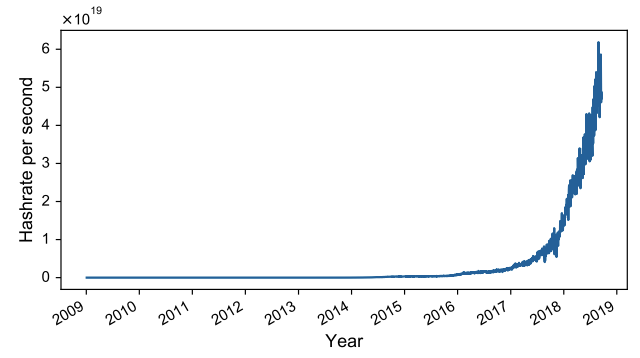
\includegraphics[width=0.55\linewidth]{images/bitcoin_hashrate.png}
    \caption{Hashrate della blockchain Bitcoin \cite{asic1}}
    \label{fig:btc-hashrate}
\end{figure}

La motivazione riconducibile a ciò è proprio l'avvento degli ASIC e la loro partecipazione al mining di Bitcoin.

Il mining basato su ASIC ha creato un picco barriera all'ingresso per il grande pubblico perché, chi interessato a minare, dovrebbe investire in attrezzature speciali per partecipare a tale processo.
A causa di ciò, come precedentemente accennato, le poche entità in grado di investire e mantenere un grande volume di ASIC potrebbero assumere il controllo della rete.
Pertanto, il mining basato su ASIC è maggiore vulnerabile all'attacco del 51\%. 


A partire da settembre 2018, i mining-pool\footnote{\textbf{Mining-pool}: minatori di criptovalute che uniscono le loro risorse per estrarre criptovalute e aumentare le probabilità di ottenere la ricompensa di un blocco} Bitcoin BTC.com e Antpool, che sono gestiti dalla stessa azienda che produce gli ASIC per la blockchain bitcoin, rappresentano oltre il 30\% del potere (hashrate) nella rete Bitcoin. 
     % TODO da ampliare

\graphicspath{{./images/}}
\section{Inizio dello sviluppo e storia
dell'algoritmo}\label{inizio-dello-sviluppo-e-storia-dellalgoritmo}

Dato che Bitcoin fallisce dal punto di vista della privacy delle
transazioni e della resistenza agli ASICs (\emph{Application Specific
Integrated Circuits}), lo sviluppatore \textbf{Nicolas van Saberhagen},
che molti pensano essere un nome di fantasia, con alcune speculazioni
che lo associerebbero al fantomatico creatore di Bitcoin,
\textbf{Satoshi Nakamoto}, nel 12 dicembre 2012 presenta un documento
con all'interno l'idea di \textbf{CryptoNote}.

Questo innovativo protocollo di consenso viene presentato come una
fattibile alternativa ai meccanismi tradizionali utilizzati dalle
criptomonete, come la \emph{Proof-Of-Work} di Bitcoin (la prova che sei
in grado di eseguire un lavoro), oltretutto in grado di garantire
elevati livelli di anonimato e un opportuna resistenza agli ASICs.
Alcune delle funzioni menzionate riguardavano transazioni di dimensione
inferiore e non facilmente associabili ad un utente, l'utilizzo delle
firme ad anello volte a migliorare la sicurezza e respingere gli
attacchi alla blockchain e l'adattamento dinamico della emissione di
moneta.

\subsection{Sviluppo dello standard CryptoNight e
adozione}\label{sviluppo-dello-standard-cryptonight-e-adozione}

Qualche mese dopo, gli sviluppatori Seigen, Max Jameson, Tuomo Nieminen,
Neocortex e Antonio M. Juarez, pubblicano un documento, facente parte
degli standard di CryptoNote, con all'interno la descrizione della
funzione di hash per la proof-of-work di CryptoNote, chiamata
\textbf{CryptoNight}.

\textbf{Bytecoin (BCN)} è stata la prima criptomoneta ad adottare il
protocollo di consenso CryptoNote, scelta giustificata dalla volontà dei
fondatori di avere una criptomoneta volta alla privacy finanziaria,
attraverso una protezione completa dell'utente che utilizza gli
strumenti finanziari messi a disposizione, dalle transazioni
all'identità personale. Come altre differenze, abbiamo l'aggiustamento
della difficoltà di minare nuova moneta ad ogni blocco, generando un
blocco ogni due minuti circa. Nonostante le buone premesse, la moneta
oggi ha un \emph{market cap} irrisorio e non è stata adottata a causa di
svariati problemi:
\begin{itemize}
  \item Inizialmente, la moneta è stata pre-minata,
  fornendo l'80\% delle monete ad un gruppo di \emph{early adopters},
  generando una distribuzione iniqua e sleale - Bytecoin ha avuto vari
  problemi tecnici di instabilità nel corso della sua vita, con difficoltà
  da parte degli utenti che partecipavano alla rete impossibilitati a
  sincronizzare tutta la blockchain.
  \item Il 20 dicembre 2017, la rete di
  Bytecoin ha ricevuto un attacco DDoS massiccio, con lo scopo di rubare
  le monete e distribuire la potenza tra le varie monete che adottano lo
  standard CryptoNote. Gli utenti affetti erano soprattutto chi aveva un
  software non aggiornato per minare nuova moneta e chi utilizzava
  \emph{desktop wallets} e \emph{web wallets} si è visto rallentare o
  disabilitare la sincronizzazione dei pagamenti, cosa che ha aumentato lo
  sconforto dei suoi partecipanti alla rete
  \item  Non si hanno notizie
  riguardo futuri sviluppi della moneta, con l'ultimo post che prometteva
  lo sviluppo di una tecnologia per nascondere gli importi delle
  transazioni e di creare un wallet più efficiente e sicuro, risalente al
  2019.
\end{itemize}

Un'altra moneta, chiamata \textbf{Monero (XMR)}, nel aprile 2014 adottò
CryptoNote, scelto per garantire la privacy e la decentralizzazione del
mining. La decisione di utilizzare questa tecnologia è stata una dei
fattori che hanno contibuito alla crescita della reputazione e al
successo di Monero come una delle monete digitali più promettenti e
utilizzate. Monero ha avuto un ruolo cruciale nello sviluppo attivo di
CryptoNight, introducendo varie modifiche al fine di adattare la
funzione alle proprie necessità. Alcune versioni utilizzate erano
specifiche per miners con risorse limitate per il mining, altre sono
state rilasciate per ottimizzare l'efficienza e l'equità del mining,
oltre a mantenere la resistenza agli ASIC. Nonostante ciò, nel 2019
Monero decise di cambiare il suo algoritmo da CryptoNote a RandomX, di
cui forniremo una descrizione data l'affinità e i prinicipi che ne
dominano lo sviluppo, oltre che risolvere una serie di problemi che si
erano sviluppati nell'algoritmo di CryptoNight.

Di seguito forniremo una panoramica sulla tecnologia CryptoNote,
presentando un approccio dettagliato e analitico per comprenderne non
solo gli aspetti funzionali e tecnici dell'algoritmo ma anche le
intrinseche necessità di migliorare lo stato corrente degli algoritmi
\emph{Proof-Of-Work}, incrementando privacy e anonimato.

\section{Aspetti tecnici di
CryptoNote}\label{aspetti-tecnici-di-cryptonote}

\subsection{Privacy e Anonimato nel Cash
Elettronico}\label{privacy-e-anonimato-nel-cash-elettronico}

Privacy e anonimato sono aspetti fondamentali del cash elettronico. I
pagamenti peer-to-peer mirano a rimanere nascosti agli occhi di terze
parti, una netta differenza rispetto alle banche tradizionali. In
generale le aziende non vogliono rivelare le loro transizioni interne e
le persone comuni desiderano mantenere riservate le proprie spese
personali.

\subsection{Proprietà di Irretracciabilità e Non
Collegabilità}\label{proprieta-di-irretracciabilita-e-non-collegabilita}

T. Okamoto e K. Ohta hanno descritto sei criteri per un sistema di
denaro elettronico ideale, uno dei quali riguarda la privacy: la
relazione tra l'utente e i suoi acquisti deve essere irrintracciabile
\cite{okamoto1991universal}. Dunque, per definire il concetto di sistema di pagamento
anonimo servono due proprietà:

\begin{itemize}
\item
  Irretracciabilità: per ogni transizione eseguita tutti i possibili
  mittenti devono avere la stessa probabilità di essere identificati.
\item
  Non collegabilità: per due qualsiasi transizioni in uscita deve essere
  impossibile dimostrare che siano state inviate dalla stessa persona
\end{itemize}

\subsection{Limiti di Bitcoin}\label{limiti-di-bitcoin}

Bitcoin non soddisfa però il primo criterio, dato che tutte le
transazioni che avvengono sono pubbliche e possono essere ricondotte a
un\textquotesingle unica origine e ad un unico destinatario.\\
Anche se due partecipanti effettuano transazioni in modo indiretto, un
metodo di ricerca del percorso ben progettato (ad esempio, l'algoritmo
``A star'' \cite{hart1968formal} può rivelare l'origine e il destinatario
finale.\\
Inoltre Bitcoin non sembra soddisfare neanche la seconda proprietà,
infatti, da un attenta analisi della blockchain e da alcune ricerche
\cite{reid2013analysis}, \cite{analysis_bitcoin}, \cite{ron2013quantitative}, si potrebbe rilevare una
connessione tra gli utenti e le loro transazioni.\\
L'incapacità di Bitcoin di soddisfare queste due proprietà porta a
concludere che esso non rappresenta un sistema anonimo, ma piuttosto
pseudo-anonimo. Sono state proposte diverse soluzioni \cite{mixing_services},
\cite{secure_multiparty} basate sull'idea di mescolare diverse transazioni pubbliche
e inviarle tramite un indirizzo intermediario ma questo porterebbe un
altro inconveniente, ovvero una terza parte fidata.

\subsection{Problemi del Protocollo di Consenso di
Bitcoin}\label{problemi-del-protocollo-di-consenso-di-bitcoin}

Il creatore di Bitcoin, Satoshi Nakamoto, ha descritto il protocollo di
consenso come ``un processore, un voto'', utilizzando SHA-256 per il
meccanismo di proof-of-work. Poiché gli utenti votano per determinare
l'ordine unico della cronologia delle transazioni, la correttezza e la
coerenza di questo processo sono condizioni fondamentali per l'intero
sistema. Ci sono due aspetti da sottolineare: - La rete è fuori pericolo
se il 51\% del potere di mining è sotto il controllo di utenti onesti. -
Il progresso del sistema è limitato perché se si vuole cambiare la
versione del protocollo il cambiamento avverrà solo se supportato dalla
stragrande maggioranza degli utenti \cite{bip_34}.

Questo permette di delineare le proprietà che una funzione di
proof-of-work deve soddisfare: non deve consentire ad un partecipante
della rete di ottenere un vantaggio significativo rispetto ad un altro,
è necesaria una sorta di equivalenza tra hardware comune e dispositivi
costisi. SHA-256 non ha queste caratteristiche: una GPU è più efficacie
di una CPU e i dispositivi ASIC sono più potenti delle GPUs
\cite{mining_hardware}.\\
Bitcoin crea quindi delle condizioni favorevoli per un ampio divario nel
potere di voto tra partecipanti, violando il principio di ``un
processore, un voto'' : i proprietari di GPU e ASIC hanno infatti molto
più potere di voto rispetto a coloro che utilizzano solo CPU.\\
\strut \\
Il sistema di script in Bitcoin è troppo complicato e pesante.
Potenzialmente consente di creare transazioni sofisticate, ma alcune
delle sue funzionalità sono disabilitate per motivi di
sicurezza\cite{contracts} \cite{script}.

\subsection{Protocolli di Firma e schemi di
CryptoNote}\label{protocolli-di-firma-e-schemi-di-cryptonote}

Seguono ora degli schemi di transazioni completamente anonime che
soddisfano le condizioni di non irretracciabilità e non collegabilità.
Una caratteristica importante è l'autonomia: il mittente non è tenuto a
collaborare con altri utenti o terze parti per le transazioni.

Lo schema di CryptoNote si basa su una primitiva crittografica chiamata
\emph{group signature}, inventata da \emph{D. Chaun} e \emph{E. van
Heyst} \cite{chaum_van_heyst} che consente di firmare un messaggio per conto di un
gruppo.\\
Dopo aver firmato, l'utente fornisce (per verificare) non la propria
chiave pubblica, ma le chiavi di tutti gli utenti del suo gruppo. Chi
verifica vede che il vero firmatario è un membro di questo gruppo, ma
non conosce la sua esatta identità.\\
Il protocollo originale prevedeva una Terza Parte Fiduciosa (Gestore del
Gruppo), ed era l'unico che poteva risalire al reale firmatario. La
versione successiva, \emph{ring} \emph{signature}, introdotta da Rivest
\cite{rivest_et_al} , prevedeva uno schema ad anello autonomo senza
responsabile del gruppo e con revoca dell'anonimato.\\
Successivamente, sono apparse diverse modifiche, quella che viene
adottata su CryptoNote per larga parte si basa sullo studio
\emph{Traceable ring signature} di \emph{E. Fujisaki and K. Suzuki}
\cite{fujisaki_suzuki}.\\
Per distinguere l\textquotesingle algoritmo originale da quello
modificato nella versione su CryptoNote, quest\textquotesingle ultima
firma verrà chiamata \emph{one-time ring signature}, sottolineando la
capacità dell\textquotesingle utente di produrre una sola firma valida
con la chiave privata.\\
La proprietà di tracciabilità è stata indebolita, mantenendo però quella
di collegabilità (linkability) per fornire unicità: la chiave pubblica
potrebbe comparire in molti set di verifica esterni e la chiave privata
può essere utilizzata per generare una firma anonima unica. Nel caso di
un tentativo di doppia spesa, queste due firme saranno collegate, ma non
è necessario rivelare l'identità del firmatario.

Alla base dell'algoritmo di firma si usa EdDSA, sviluppato e
implementato da \emph{D.J. Bernstein} \cite{bernstein_et_al}, parametri comuni di
dominio sono: - q: numero primo; - d: elemento of Fq; - E: equazione
della curva ellittica; - G: punto base; - l: ordine primo del punto
base; - Hs: funzione hash crittografica \{0, 1\} * → Fq; - Hp: funzione
hash deterministica E(Fq) → E(Fq).

Al fine di ottenere una maggiore privacy, sono necessari alcuni nuovi
termini che non dovrebbero essere confusi con le entità di Bitcoin:

\begin{itemize}
  \item
    \textbf{private ec-key} è una chiave segreta standard di curva
    ellittica: un numero $a \in [1,l-1]$
  \item
    \textbf{public ec-key} è una chiave pubblica standard di curva
    ellittica: un punto $A=aG$;
  \item
    \textbf{one-time keypair} è una coppia di chiavi ec-private e
    ec-public;
  \item
    \textbf{private user key} è una coppia \emph{$(a, b)$} di due diverse
    chiavi ec-private;
  \item
    \textbf{tracking key} è una coppia \emph{$(a, B)$} di chiave ec-private
    e chiave ec-public \emph{(dove $B=bG$ e $a \neq b$)};
  \item
    \textbf{public user key} è una coppia \emph{$(A, B)$} di due chiavi
    ec-public derivate da \emph{$(a, b)$};
  \item
    \textbf{standard} \textbf{address} è una rappresentazione di una
    chiave utente pubblica mediante una stringa digitabile
    dall\textquotesingle utente con correzione degli errori.
  \end{itemize}

La struttura generale della transazione rimane quasi identica a quella
di Bitcoin: ogni utente può scegliere diversi pagamenti (transaction
outputs), firmarli con le chiavi private corrispondenti e inviarli a
diverse destinazioni.\\
Contrariamente al modello di Bitcoin, in cui un utente possiede sia le
chiavi uniche private che pubbliche, nel modello proposto un mittente
genera una chiave one-time publica basata sull'indirizzo del
destinatario e su alcuni dati. In questo senso, una transazione in
entrata per lo stesso destinatario viene inviata a una chiave pubblica
monouso (non direttamente a un indirizzo univoco) e solo il destinatario
può recuperare la parte privata corrispondente per riscattare i suoi
fondi (utilizzando la sua chiave privata unica). Il destinatario può
spendere usando una firma ad anello, mantenendo anonima la sua proprietà
e la sua effettiva spesa.

\subsection{Funzionamento delle
transazioni}\label{funzionamento-delle-transazioni}

Gli indirizzi Bitcoin classici, una volta pubblicati, diventano
identificatori inequivocabili per ogni pagamento in entrata,
collegandoli tra loro e associandoli al destinatario.

\begin{figure}[h]
  \centering
  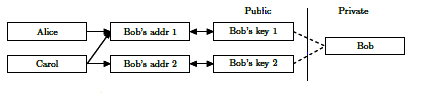
\includegraphics[width=0.5\textwidth]{image6.png}
  \caption{Modello chiave/transazione tradizionale di Bitcoin.}
  \label{fig:my_label}
\end{figure}

Viene proposta una soluzione che consente all\textquotesingle utente di
pubblicare un singolo indirizzo e ricevere pagamenti incondizionati non
collegabili. La destinazione di ciascun output (di default) è una chiave
pubblica unica, derivata dall\textquotesingle indirizzo del destinatario
e dall\textquotesingle iniezione di dati casuali da parte del
mittente.\\

\begin{figure}[h]
  \centering
  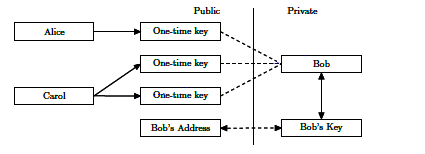
\includegraphics[width=0.5\textwidth]{image7.png}
  \caption{Modello di transazione CryptoNote.}
  \label{fig:my_label}
\end{figure}

Innanzitutto, il mittente esegue il protocollo di scambio Diffie-Hellman
per ottenere un segreto condiviso dai suoi dati e da una metà
dell\textquotesingle indirizzo. Successivamente calcola una chiave di
destinazione monouso, utilizzando questi segreti e la seconda metà. Per
questi due passaggi sono necessarie due chiavi ec-keys del destinatario;
quindi, un indirizzo CryptoNote standard è grande quasi il doppio di un
indirizzo Bitcoin. Il destinatario esegue anche il protocollo
Diffie-Hellman e poi recupera la chiave segreta corrispondente.

Una transazione standard procede come segue:

\begin{enumerate}
\def\labelenumi{\arabic{enumi}.}
\item
  Alice vuole inviare un pagamento a Bob, che ha pubblicato il suo
  indirizzo. Lo decomprime e ottiene la chiave utente pubblica di Bob
  \emph{$(A, B)$}.
\item
  Alice genera un numero casuale $r \in [1,l-1]$ e calcola la chiave
  pubblica one-time $P=H_s(rA)G+B$.
\item
  Alice usa $P$ come chiave di destinazione per l\textquotesingle output e
  inserisce anche il valore $R=rG$ (come parte del protocollo
  Diffie-Hellman) da qualche parte nella transazione. Alice può creare
  altri output con chiavi pubbliche uniche: chiavi diverse dei
  destinatari \emph{$(A_i,B_i)$} implicano $P_i$ diversi anche con
  lo stesso $r$.

  \begin{figure}[h]
    \centering
    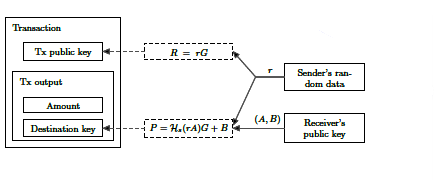
\includegraphics[width=0.5\textwidth]{image3.png}
    \caption{Standard transaction structure.}
    \label{fig:my_label}
  \end{figure}
\item
  Bob controlla ogni transazione in arrivo con la sua chiave privata $(a,
  b)$, calcolando $P'=H_s(aR)G+B$. Se la transazione di Alice è presente,
  allora $aR=arG=rA$ e $P'=P$.
\item
  Ora Bob può recuperare la chiave privata una tantum corrispondente:
  $x=H_s(aR)+b$, così come $P=xG$. Può spendere questo output in qualsiasi
  momento firmando la transazione con $x$.

  \begin{figure}[h]
    \centering
    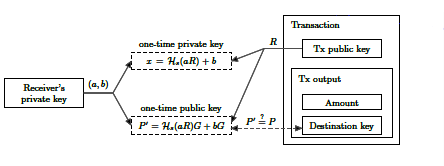
\includegraphics[width=0.5\textwidth]{image4.png}
    \caption{Check della transazione in ingresso.}
    \label{fig:my_label}
  \end{figure}
\end{enumerate}

Di conseguenza, Bob riceve pagamenti in entrata associati a chiavi
pubbliche monouso che non possono essere collegate per un osservatore
esterno.

\subsubsection{Firme ad anello}\label{firme-ad-anello}

Un protocollo basato su firme ad anello monouso consente agli utenti di
ottenere un\textquotesingle anonimato incondizionato. Purtroppo, i tipi
ordinari di firme crittografiche permettono di tracciare le transazioni
ai rispettivi mittenti e destinatari. La \emph{one-time ring signature}
usa diverse tipi di firme, consiste di quattro algoritmi (\textbf{GEN,
SIG, VER, LNK}).

\begin{itemize}
  \item
    \textbf{GEN} prende parametri pubblici e restituisce una coppia ec
    \emph{$(P, x)$} e una chiave pubblica $I$.
  \item
    \textbf{SIG} riceve un messaggio $m$, un insieme $S'$ di chiavi pubbliche
    $\{P_i\}_{i \neq s}$, le coppie \emph{$(P_s, x_s)$} e restituisce una firma $\sigma$ e un
    insieme $S = S' \cup \{P_s\}$.
  \item
    \textbf{VER} riceve un messaggio $m$, un insieme $S$, una firma $\sigma$ e
    restituisce "true" o "false".
  \item
    \textbf{LNK} riceve un insieme $I = \{I_i\}$, una firma $\sigma$ e restituisce
    "linked" o "indep".
\end{itemize}

Lo scopo principale del protocollo è il seguente: un utente produce una
firma che può essere verificata non da una singola chiave pubblica, ma
da un insieme di chiavi. Il vero firmatario è indistinguibile dagli
altri proprietari di chiavi fino a quando non produce la seconda firma
sotto la stessa coppia di chiavi.

\begin{figure}[h]
  \centering
  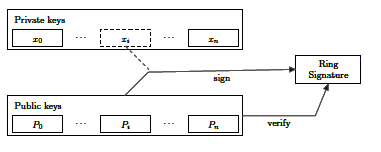
\includegraphics[width = 0.55\textwidth]{image5.png}
  \caption{Anonimità firme ad anello.}
\end{figure}

\begin{itemize}
  \item
    \textbf{GEN}: Il firmatario sceglie casualmente una chiave segreta $x \in
    [1,l-1]$ e calcola la chiave pubblica corrispondente $P=xG$. Inoltre,
    calcola un\textquotesingle altra chiave pubblica $I=xHp(P)$ chiamata
    "immagine della chiave".
  \item
    \textbf{SIG}: Il firmatario genera una firma ad anello one-time con
    una prova a conoscenza zero non interattiva. Seleziona un sottoinsieme
    casuale $S'$ di $n - 1$ chiavi pubbliche di altri utenti $P_i$,
    la propria coppia di chiavi $(x, P)$ e l\textquotesingle immagine della
    chiave $I$. Sia $1 \leq s \leq n$ l\textquotesingle indice segreto del firmatario in
    $S$ (in modo che la sua chiave sia $P_s$).\\
    Si sceglie casualmente un elemento casuale da $\{q_i | i = 1
    ... n\}$ e $\{w_i | i = 1 ... n, i \neq s\}$ da $(1 ... l)$ e effettua
    i seguenti passaggi:
    \[ L_i = \begin{cases} q_iG, & \text{se } i = s \\ q_iG+w_iP_i, & \text{se } i \neq s \end{cases} \]


\[ R_i = \begin{cases} q_iH_p(P_i), & \text{se } i = s \\ q_iH_p(P_{i})+ w_iI, & \text{se } i \neq s \end{cases} \]

Il prossimo passo è ottenere la sfida non interattiva:

\[ c = H_s(m, L_1, \ldots, L_n, R_1, \ldots, R_n) \]

Infine il firmatario calcola la risposta:

\[ c_i = \begin{cases} w_i, & \text{se } i \neq s \\ \left(c -\sum_{i=1}^{n} c_i\right) \mod l, & \text{se } i = s \end{cases} \]

\[ r_i = \begin{cases} q_i, & \text{se } i \neq s \\ q_s - c_sx \mod l ,& \text{se } i=s \end{cases} \]

La firma risultante è \[ \sigma= (I,c_1,\ldots,c_n,r_1,\ldots,r_n). \]

\item 
  \textbf{VER}: Chi sta verificando controlla la firma, ricostruendo:

\[ \begin{cases}
L_i' = r_iG + c_iP_i \\
R_i' = r_iH_p(P_i) + c_iI
\end{cases}
 \] Chi verifica controlla se
\[\sum_{i=1}^{n} ci =^? H_s(m,L_1',...,L_n',R_1',...R_n') \mod l \]

Se questa uguaglianza è vera, chi verifica esegue
l\textquotesingle algoritmo \textbf{LNK}, altrimenti respinge la firma.
\item 
  \textbf{LNK}: Chi verifica controlla se I è stata utilizzata in firme
passate (questi valori sono memorizzati nell\textquotesingle insieme I).
Un doppio utilizzo significa che sono state prodotte due firme con la
stessa chiave segreta.\\
\end{itemize}
Meccanismo del protocollo: utilizzando L-commitments, il firmatario
dimostra di conoscere un certo $x$ tale che almeno una $Pi = xG$.
Per rendere
questa prova non ripetibile introduciamo l\textquotesingle immagine
della chiave come $I=xHp(P)$. Il firmatario utilizza gli stessi
coefficienti $(r_i,c_i)$ per dimostrare quasi la stessa cosa: egli conosce
un certo $x$ tale che almeno uno $Hp(P_i)=I \cdot x^{-1}$. Se $x \rightarrow I$ è iniettiva:

\begin{itemize}
\item 
  Nessuno può recuperare la chiave pubblica dall\'immagine della chiave e identificare il firmatario.
\item 
  Ilfirmatario non può fare due firme con I diverse e lo stesso x.
\end{itemize}

Con una firma ad anello one-time, Bob può efficacemente nascondere
l'output di Alice (cioè, il suo input) tra gli altri: tutti i possibili
spenditori saranno equiprobabili, anche se Alice non ha più informazioni
di qualsiasi osservatore. Bob specifica n-1 outputs, non sapendo se
alcuni di questi sono stati spesi:\\
Un output può essere utilizzato in migliaia di firme come fattore di
ambiguità e mai come obiettivo di occultamento. Il controllo di doppia
spesa avviene nella fase LNK quando si cerca
nell\textquotesingle insieme delle immagini di chiave utilizzate.\\
Bob può scegliere il grado di ambiguità autonomamente: n = 2 significa
che avrà speso l\textquotesingle output con una probabilità del 50\%, n
= 100 dà il 1\%. La dimensione della firma risultante è lineare O(n),
quindi l\textquotesingle anonimato costa a Bob una dimensione di
transazione più grande e commissioni più alte.

Combinando entrambi i metodi (chiavi di transazione one-time e firme ad
anello one-time), Bob raggiunge un nuovo livello di privacy rispetto
allo schema originale di Bitcoin. Gli basta memorizzare una sola chiave
privata (a, b) e generare una chiave pubblica (A, B) per iniziare a
ricevere e inviare transazioni anonime. Per ogni output Bob recupera
coppie di chiavi di transazione uniche (pi, Pi) che non possono essere
collegate tra loro o alla sua chiave pubblica. Può spendere ognuna di
esse, firmando ogni input con una firma ad anello non tracciabile.

\subsection{Miglioramenti nella PoW rispetto a
Bitcoin}\label{miglioramenti-nella-pow-rispetto-a-bitcoin}

C'è stato anche un miglioramento dell'algoritmo di PoW, come obiettivo
primario vi è l'abbassamento del gap tra CPU e GPU/FPGA/ASIC.\\
Il protocollo originale di proof-of-work di Bitcoin utilizza la funzione
SHA-256.\\
Consiste principalmente di operatori logici di base e si basa
esclusivamente sulla velocità computazionale del processore, quindi è
perfettamente adatto per l\textquotesingle implementazione
multicore/conveyer. Tuttavia, i computer moderni non sono limitati solo
dal numero di operazioni al secondo, ma anche dalla dimensione della
memoria. Mentre alcuni processori possono essere notevolmente più veloci
di altri \cite{mining_hardware}, le dimensioni della memoria sono meno probabili
che varino tra le macchine.\\
L\textquotesingle idea principale è costruire un algoritmo che alloca un
ampio blocco di dati ("scratchpad") all\textquotesingle interno della
memoria e "accedere a una sequenza imprevedibile di posizioni" in esso.
Il blocco dovrebbe essere sufficientemente grande per rendere più
vantaggioso conservare i dati piuttosto che ricalcolarli ad ogni
accesso. L\textquotesingle algoritmo dovrebbe inoltre impedire il
parallelismo interno, quindi N thread simultanei dovrebbero richiedere N
volte più memoria contemporaneamente.\\
\emph{Dwork et al} \cite{dwork_et_al} hanno investigato e formalizzato questo
approccio, portandoli a suggerire un\textquotesingle altra variante
della funzione di pricing: "Mbound". Un altro lavoro appartiene a \emph{F.
Coelho} \cite{coelho}, che ha proposto la soluzione più efficace:
"Hokkaido". Con ogni probabilità, l\textquotesingle ultimo lavoro è
basato sull\textquotesingle idea di ricerche pseudo-casuali in un grande
array è l\textquotesingle algoritmo noto come \emph{scrypt} di \emph{C. Percival}
\cite{percival}. A differenza delle funzioni precedenti, si concentra sulla
derivazione delle chiavi e non sui sistemi di proof-of-work. Nonostante
ciò, scrypt funziona bene come funzione di prezzo nel problema di
conversione dell'hash parziale come SHA-256 in Bitcoin.\\
Per ora lo script è stato applicato a Litecoin \cite{litecoin}, ma la sua
implementazione non è veramente legata alla memoria: il rapporto ``tempo
di accesso alla memoria / tempo complessivo'' non è abbastanza grande
perché ogni istanza utilizza solo 128 KB, questo dunque permette ai
miner GPU di essere 10 volte più efficienti lasciando la possibilità di
creare dispositivi di mining efficienti e relativamente economici.\\
CryptoNote propone quindi un nuovo algoritmo memory-bound per la
proof-of-work. Si basa sull\textquotesingle accesso casuale a una
memoria lenta e sottolinea la dipendenza dalla latenza. A differenza di
scrypt, ogni nuovo blocco (lungo 64 byte) dipende da tutti i blocchi
precedenti e non solo da uno, quindi il compromesso tra dimensione della
memoria e velocità della CPU diventa esponenziale. Il nuovo algoritmo
richiede circa 2 Mb per istanza per i seguenti motivi:

\begin{itemize}
\item
  Si adatta alla cache L3 (per core) dei processori moderni, che
  diventeranno mainstream tra qualche anno;
\item
  Un megabyte di memoria interna è quasi una dimensione inaccettabile
  per il moderno pipeline ASIC;
\item
  Le GPU possono eseguire centinaia di istanze simultanee, ma sono
  limitate in altri modi: la memoria GDDR5 è più lenta della cache L3
  della CPU e notevole per la sua larghezza di banda, non per la
  velocità di accesso casuale.
\item
  Un\textquotesingle espansione significativa dello scratchpad
  richiederebbe un aumento delle iterazioni, il che implica a sua volta
  un aumento del tempo complessivo. Chiamate "pesanti" in una rete P2P
  senza fiducia possono portare a gravi vulnerabilità, perché i nodi
  sono obbligati a verificare il proof-of-work di ogni nuovo blocco. Se
  un nodo impiega una quantità considerevole di tempo per ogni
  valutazione dell\textquotesingle hash, può essere facilmente soggetto
  a attacchi DDoS da parte di una valanga di oggetti falsi con dati di
  lavoro arbitrari (valori di nonce).
\end{itemize}

\subsection{Equità nella
distibuzione}\label{equituxe0-nella-distibuzione}

Il limite superiore per l\textquotesingle ammontare complessivo delle
monete digitali CryptoNote è anche digitale:
\[\text{MSupply} = 2^{64} - 1\] unità atomiche. Questa è una restrizione
naturale basata solo su limiti di implementazione, non su intuizioni
come "N monete dovrebbero essere sufficienti per chiunque".

Per garantire la regolarità del processo di emissione, viene utilizzata
la seguente formula per le ricompense dei blocchi: \[
\text{BaseReward} = (\text{MSupply} - A) >> 18 \]

dove A è l\textquotesingle ammontare di monete generate precedentemente

CryptoNote contiene un algoritmo di targeting che cambia la difficoltà
di ogni blocco. Questo migliora il tempo di reazione del sistema quando
la potenza di calcolo della rete cresce o diminuisce intensamente,
preservando un tasso di blocco costante. Il metodo originale di Bitcoin
calcola il rapporto tra la difficoltà effettiva e quella target tra gli
ultimi 2016 blocchi e lo utilizza come moltiplicatore per la difficoltà
attuale. Ovviamente questo è inadatto per ricalcoli rapidi (a causa
dell\textquotesingle inerzia elevata) e porta a oscillazioni.
L\textquotesingle idea generale dietro l'algoritmo è sommare tutto il
lavoro completato dai nodi e dividerlo per il tempo impiegato per
completare il lavoro. La misura del lavoro sono i valori di difficoltà
corrispondenti in ogni blocco.

Gli utenti pagano gli altri per memorizzare la blockchain e dovrebbero
avere il diritto di votare per la sua dimensione. Ogni miner si
confronta con il compromesso tra bilanciare i costi e il profitto dalle
commissioni, quindi stabilisce il proprio "limite flessibile" per la
creazione dei blocchi. Inoltre, la regola fondamentale per la dimensione
massima del blocco è necessaria per evitare che la blockchain venga
inondatata da transazioni fasulle, tuttavia questo valore non dovrebbe
essere codificato duramente. Sia MN il valore mediano delle dimensioni
degli ultimi N blocchi.\\
Allora il "limite rigido" per la dimensione dei blocchi accettati è 2 ·
MN.

Un miner ha ancora la possibilità di riempire un blocco con le sue
transazioni senza commissioni fino alla dimensione massima di 2 MB.
Anche se solo la maggioranza dei miners può spostare il valore mediano,
esiste comunque la possibilità di gonfiare la blockchain e produrre un
carico aggiuntivo sui nodi. Per scoraggiare i partecipanti malevoli dal
creare blocchi grandi, introduciamo una funzione di penalità:

\[
\text{NewReward} = \text{BaseReward} \times \left( \frac{\text{DimBlocco}}{MN} - 1 \right)^2
\]

Questa regola viene applicata solo quando la DimBlocco è maggiore della
dimensione minima del blocco gratuito che dovrebbe essere vicina a \[
\max(10\, \text{kb}, M_N \cdot 110\%) \] I miners sono autorizzati a
creare blocchi di ``dimensioni usuali'' e persino a superarle con
profitto quando le commissioni complessive superano la penalità.\\
Tuttavia, è improbabile che le commissioni crescano in modo quadratico a
differenza del valore della penalità, quindi ci sarà un equilibrio.
       % TODO non c'è un nuovo chapter, quindi al di là del nome al momento finisce nell'introduzione. io lo lascerei così
\chapter{CryptoNight}
\section{Introduzione alle PoW ASIC-resistant}
Al fine di scoraggiare l'uso di sistemi basati su ASIC per il mining, citati nel primo capitolo, sono stati proposti diversi meccanismi PoW ASIC-resistant.
I principali algoritmi di questo tipo possono essere divisi in: PoW Multi-hash, PoW Memory-hard e PoW Programmatic.

\subsection{PoW Multi-hash}
A differenza dell'algoritmo PoW di Bitcoin che utilizza solo un tipo di funzione hash, gli algoritmi PoW Multi-hash impiegano più funzioni hash per calcolare la validità del blocco. Queste funzioni hash vengono applicate all'intestazione del blocco in una sequenza, che può essere fissa o determinata dinamicamente per ogni blocco. 
Alcuni degli algoritmi PoW multi-hash più famosi sono: \textit{X11, X14, X17, X11EVO, X16S, X16R, Quark} e \textit{TimeTravel}.

Nella ricerca scientifica di Cho, dal titolo "\textit{ASIC-Resistance of Multi-Hash Proof-of-Work Mechanisms for Blockchain Consensus Protocols}" \cite{asic1}, è stato dimostrato come gli algoritmi multi-hash non hanno una significativa differenza da altri meccanismi PoW semplici.
Inoltre, nonostante gli algoritmi di questa categoria siano spesso definiti ASIC-resistance, alcuni di loro sono già stati rotti da sistemi ASIC.
Mentre, per quanto riguarda gli algoritmi rimanenti, non è stato mai dimostrato se siano veramente resistenti agli ASIC o se semplicemente non sono ancora stati progettati ASIC specifici per essi, magari in quanto impiegati in reti piccole dal basso valore economico.

Dati i risultati ottenuti, nel paper si suggerisce di optare per l'impiego di altri meccanismi ASIC-resistant per scoraggiare effettivamente il mining basato su ASIC.

\subsection{Programmatic PoW}
Una delle nuove direzioni per meccanismi PoW resistenti è aumentare la diversità delle computazioni. 
Nell'approccio PoW Programmatic, il processo di mining coinvolge l'esecuzione di un programma che cambia frequentemente. 
Ad esempio, aggiungendo come parte della computazione un pool di funzioni matematiche o un programma generato casualmente. 

Questo rende difficile per gli ASIC ottimizzare il mining, poiché dovrebbero essere riprogrammati ogni volta che il programma cambia.
Sarebbe impraticabile costruire moduli hardware specializzati che mirino a ciascuna delle possibili attività di calcolo.  

Questo tipo di meccanismi PoW sono in fase di studio e non sono ancora stati utilizzati per la realizzazione di una vera e propria blockchain.


\subsection{PoW Memory-hard}
Infine, sebbene gli ASIC offrano una maggiore efficienza computazionale rispetto alle piattaforme di calcolo general-purpose, sono solitamente limitati in termini di memoria.
    
In un algoritmo PoW Memory-hard, il processo di mining richiede l'utilizzo di grandi quantità di memoria per importare dati complessi e calcolarne l'hash.
Una computazione in questi algoritmi richiederà il recupero di dati casuali da un grande set di dati. 
La dimensione dell'insieme sarà sufficientemente grande da rendere difficile la progettazione di un ASIC che memorizzi tutto in una memoria on-chip.

Gli algoritmi PoW memory-hard più conosciuti sono: \textit{Ethash} di Ethereum, \textit{Scrypt} e \textit{CryptNight}. 

Ad esempio, per l'algoritmo di consenso \textit{Ethash}, utilizzato nella blockchain Ethereum, 
è stato sviluppato l'ASIC Antminer E3 che ha un hash rate di 190 MH/s, che è solo 2 volte più 
veloce della GPU V100, a fronte di un consumo energetico 3 volte superiore.
Sottolineando come i processori specializzati (ASIC e FPGA) hanno un vantaggio minimo rispetto 
alle CPU e GPU a causa della complessità degli algoritmi e dell'elevato costo della memoria. 




\subsubsection{Introduzione alla Memory-Hardness di CryptoNight}
CryptoNote propone quindi CryptoNight, sul quale si entrerà in dettaglio nella prossima sezione, 
come algoritmo PoW che assicura la Memory-Hardness.
Tale proprietà è garantita grazie ad un ciclo che esegue una sequenza di letture e scritture casuali 
in una piccola area di memoria da 2MB, chiamata \textit{scratchpad}. 

L'algoritmo CryptoNight si compone di tre fasi principali:
inizializzazione dello scratchpad, il memory-hard loop ed un calcolo finale del risultato.

Nella fase 2 del loop i passaggi elencato nell'Algoritmo e nell'immagine in Figura \ref{fig:cryptonight-loop}. 
\begin{itemize}
    \item Sia A che B sono interi a 16 byte e vengono inizializzati con il risultato XOR dei byte da 0 a 31 e da 32 a 63 generati utilizzando la funzione Keccak. 
    \item Questi interi vengono quindi utilizzati come indirizzi nello scratchpad analizzando i 21 bit meno significativi. 
    Si legge il valore S[A] nello scratchpad usando A come indirizzo e si esegue la crittografia AES di S[A] con A per ottenere il risultato C. 
    \item Successivamente si esegue lo XOR su B e C e si riscrive il risultato XOR in S[A]. Si usa poi C come indirizzo, si legge S[C] in D, si moltiplicano C e D, si aggiunge il risultato della moltiplicazione ad A e si memorizza A in S[C].
    \item Infine, si ottiene il risultato XOR di A e D come nuovo A, e C come nuovo B, e si utilizeranno il nuovo A e B all'iterazione successiva. 
\end{itemize}

\begin{figure}[h!]
    \centering
    \makebox[\textwidth][c]{
    
        \begin{minipage}{0.5\linewidth}
            \centering
            \begin{algorithm}[H]
            \caption{}
            \begin{algorithmic}[1]
            \Require Integer $A$, $B$, Scratchpad memory $S$
            \Ensure Modified scratchpad memory $S$
            \For{$i \leftarrow 1$ to $524288$}
                \State $C \leftarrow \text{AES}(S[A], A)$
                \State $S[A] \leftarrow \text{XOR}(B, C)$
                \State $D \leftarrow S[C]$
                \State $A \leftarrow \text{ADD}(A, \text{MUL}(C, D))$
                \State $S[C] \leftarrow A$
                \State $A \leftarrow \text{XOR}(A, D)$
                \State $B \leftarrow C$
            \EndFor
            \end{algorithmic}
            \end{algorithm}
        \end{minipage}
        
        \hspace{0.05\linewidth}
        
        \begin{minipage}{0.45\linewidth}
            \centering
            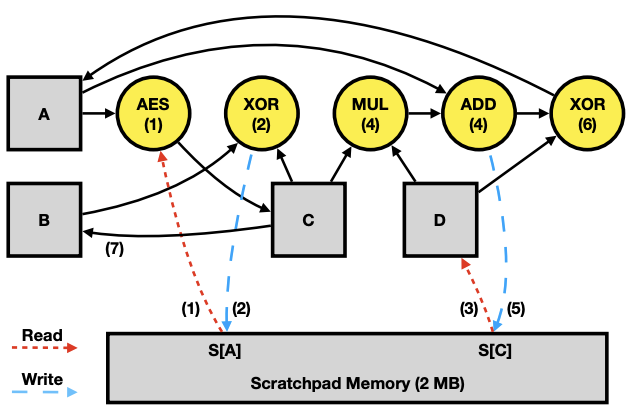
\includegraphics[width=\linewidth]{images/cryptonight.png}
        \end{minipage}
    }
    \caption{Memory-Hard loop dell'algoritmo CryptoNight. \cite{asic_memory_hard}}
    \label{fig:cryptonight-loop}
\end{figure}

Una parte del ciclo utilizza la crittografia AES per generare indirizzi di memoria casuali ai quali poi accedere.
Poiché l'output di AES è intrinsecamente casuale, non è possibile prevedere in anticipo quale sarà l'indirizzo 
di memoria successivo da leggere o scrivere. Questo impedisce la parallelizzazione del ciclo di operazioni di 
lettura e scrittura, poiché ogni iterazione dipende dal risultato dell'iterazione precedente.

Il ciclo di CryptoNight prevede 524.288 iterazioni. 
Durante ogni iterazione, viene effettuata una lettura e una scrittura casuale nello "scratchpad". 
Pertanto, l'intero ciclo comporta circa 2 milioni di operazioni di lettura e scrittura casuali. 
Questa caratteristica rende CryptoNight resistente agli attacchi con hardware specializzato come gli ASIC, 
che solitamente sfruttano la parallelizzazione per aumentare l'efficienza del mining.


\subsubsection{Risultati sperimentali}
Nel paper intitolato "\textit{Evaluating Memory-Hard Proof-of-Work Algorithms on Three Processors}" \cite{asic_memory_hard}, Feng e Luo confrontano tra loro \textit{CryptoNight}, \textit{Ethash}, \textit{Hashcash} e \textit{Cuckoo} su CPU, GPU e KNL, giungendo alla conclusione che la Memory-Hardness può essere raggiunta sfruttando la latenza o la bandwith.

I compiti che dipendono dalla latenza sono più adatti per CPU, grazie alla loro gerarchia di cache ben sviluppata. 
Al contrario, i compiti che richiedono una grande larghezza di banda possono sfruttare appieno il potenziale delle GPU.

Nel caso di studio, CryptoNight implementa una resistenza alla memoria mediante la latenza, sfruttando il tempo di accesso alla memoria per rendere più difficile la creazione di hardware specializzato.

Tuttavia, come seconda considerazione, viene specificato che, poiché i processori si stanno evolvendo rapidamente, gli algoritmi di Proof-of-Work dovrebbero essere adattabili e flessibili affinché le loro proprietà possano essere mantenute il più a lungo possibile. 



\subsection{La vittoria degli ASIC su CryptoNight}
CryptoNight rimase immune agli ASIC per un lungo periodo. Tuttavia, a partire dal 2018 vennero annunciati diversi modelli di ASIC per CryptoNight (Bitmain, Baikal e Halong Mining), capaci di raggiungere un hashrate superiore ai 200 KH/s.


\subsubsection{Bitmain}
Il 15 marzo 2018, Bitmain, un'azienda cinese, ha annunciato l'Antminer-X3, un ASIC progettato appositamente per il mining di criptovalute basate su CryptoNight. Secondo le specifiche riportate sul sito di Bitmain, l'X3 ha un tasso di hash totale di 220 kH/s e un consumo energetico di 465W.

È interessante notare la risposta su Twitter del responsabile del progetto Monero all'epoca, Riccardo Spagni, il quale sottolinea l'inefficacia dell'Antminer-X3 per la blockchain di Monero (Figura \ref{fig:Antminer-X3}).
Al tempo Monero utilizzava come PoW proprio CryptoNight, tuttavia come parte del suo protocollo blockchain adotta regolarmente hard fork pianificati e di emergenza al fine di mitigare qualsiasi potenziale minaccia derivante dagli ASIC.

% https://www.getmonero.org/2018/02/11/PoW-change-and-key-reuse.html

\begin{figure}[h!]
    \centering
    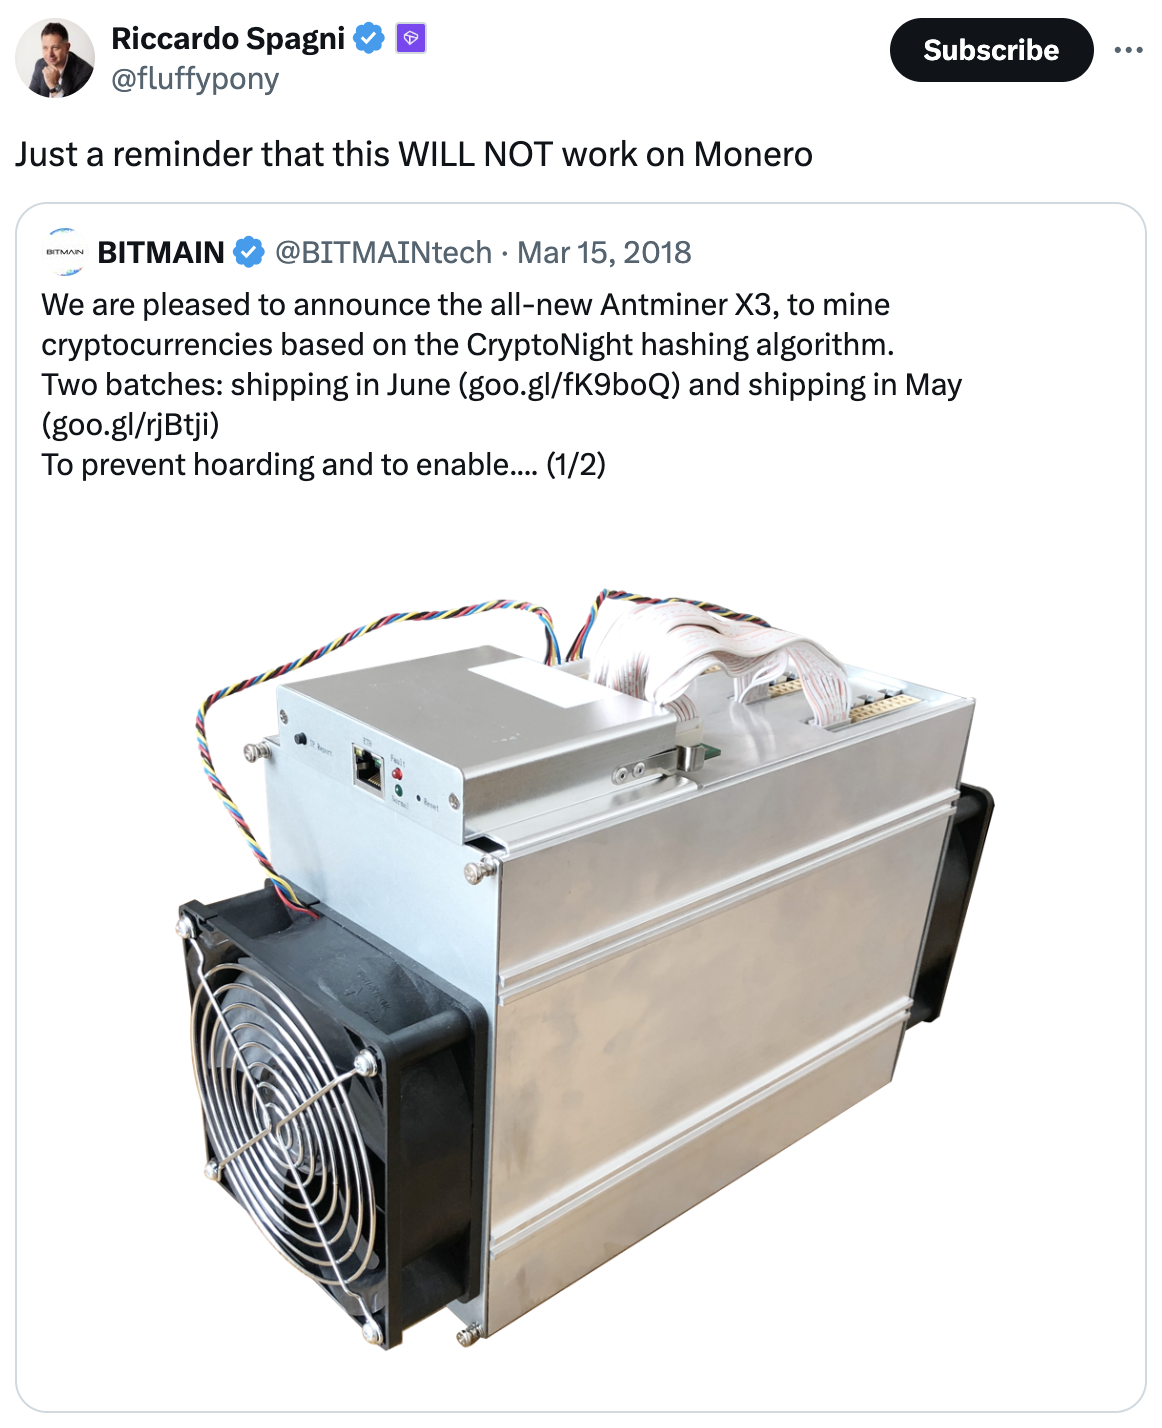
\includegraphics[width=0.45\linewidth]{images/Antminer-X3.png}
    \caption{Modello Antminer-X3 (Bitmain)}
    \label{fig:Antminer-X3}
\end{figure}

La strategia adottata da Monero gli conferisce immunità agli ASIC come l'X3 e quelli che presentati nelle prossime sezioni. 
Tuttavia, tali dispositivi rimangono utili per il mining di altre criptovalute basate su CryptoNight, come Bytecoin, Dinastycoin, Karbo e vecchie fork di Monero, che non implementano misure simili.



\subsubsection{Baikal}
Anche la società russa Baikal Mining ha reagito prontamente, rilasciando un primo modello meno potente nello stesso mese del concorrente cinese e un secondo modello più performante alcuni mesi dopo.
Entrambi gli ASIC sono in grado di minare gli algoritmi CryptoNight e CryptoNight-Lite.

\begin{itemize}
    \item[(a)] Modello BK-N, rilasciato nel marzo 2018 con un hashrate massimo di 80 kH/s ed un consumo di 120W (Figura \ref{fig:Baikal BK-N}),
    \item[(b)] Modello BK-N240, rilasciato nel maggio 2018 con un hashrate massimo di 480 kH/s ed un consumo di 650W (Figura \ref{fig:Baikal N240}).
\end{itemize}

\begin{figure}[h!]
    \centering
    \begin{subfigure}[b]{0.15\linewidth}
        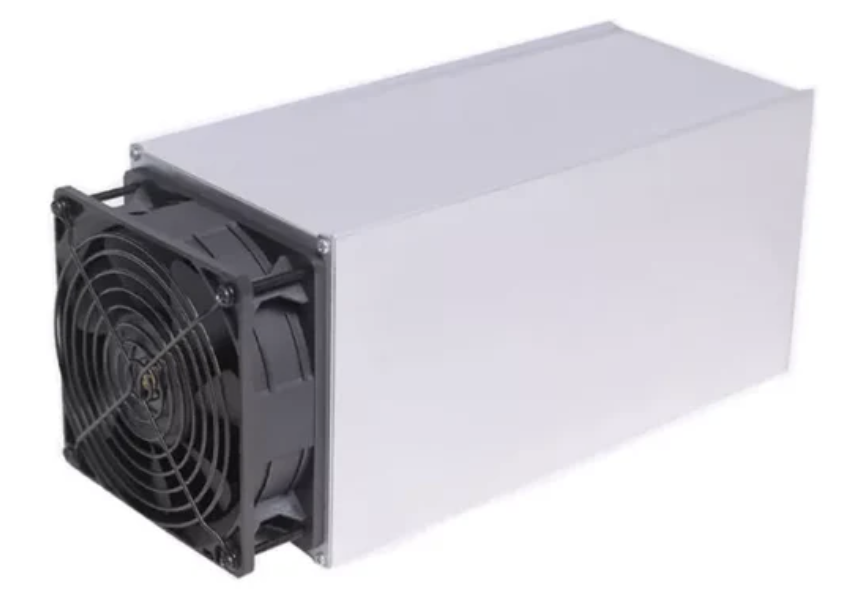
\includegraphics[width=\linewidth]{images/Baikal BK-N.png}
        \caption{}
        \label{fig:Baikal BK-N}
    \end{subfigure}
    \hspace{1.5cm}
    \begin{subfigure}[b]{0.15\linewidth}
        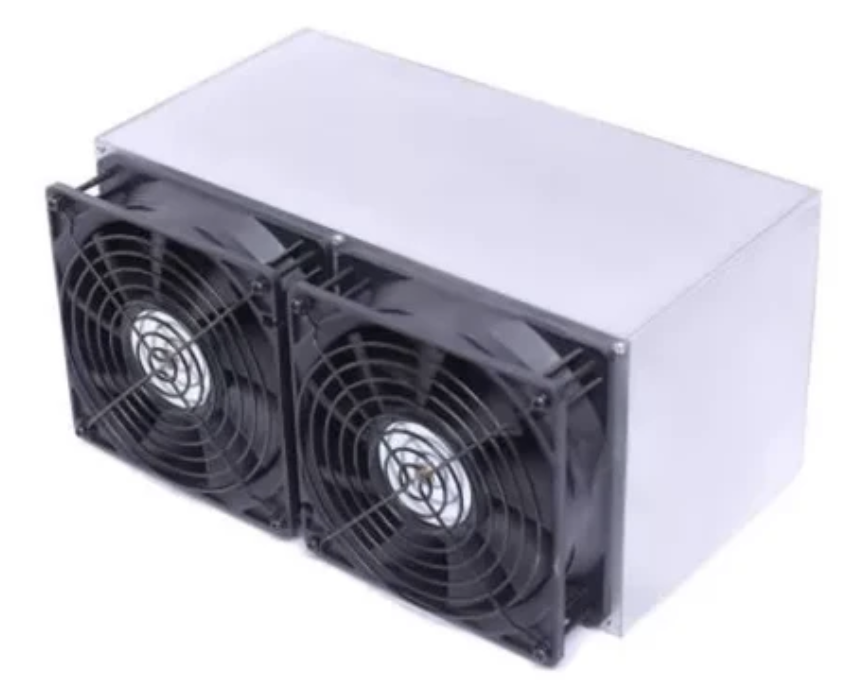
\includegraphics[width=\linewidth]{images/Baikal N240.png}
        \caption{}
        \label{fig:Baikal N240}
    \end{subfigure}
    \caption{Modelli ASICS BK-N e BK-N240 (Baikal)}
    \label{fig:Baikal miners}
\end{figure}


\subsubsection{Halong Mining}
Con un mese di ritardo, nell'Aprile 2018, anche l'azienda statunitense Halong Mining ha rilasciato il suo Modello DragonMint X2, in grado di minare l'algoritmo CryptoNight con un hashrate massimo di 248 kH/s e un consumo energetico di 490W.

\begin{figure}[h!]
    \centering
    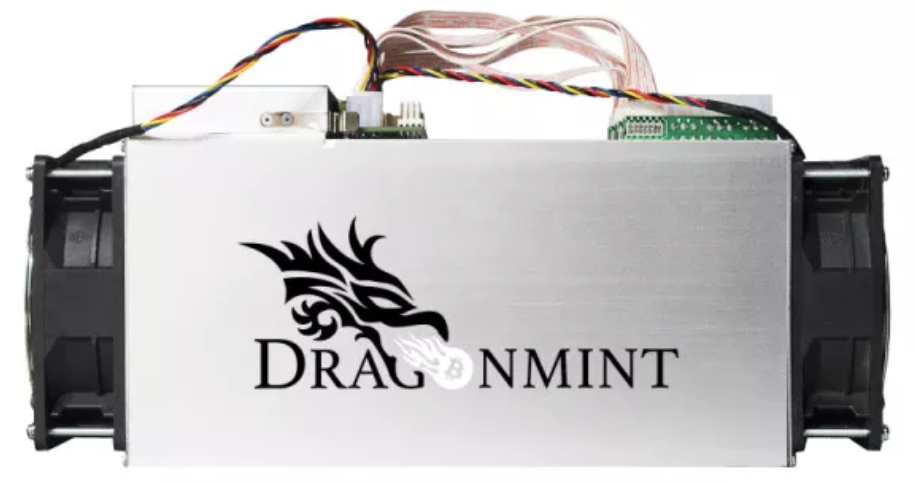
\includegraphics[width=0.2\linewidth]{images/DragonMint X2.png}
    \caption{Modello ASICS DragonMint X2 (Halong Mining)}
\end{figure}



\section{Funzione di hash CryptoNight}\label{funzione-di-hash-cryptonight}
In questa sezione si parlerà del cuore del protocollo di consenso
CryptoNote, la funzione di hash \textbf{CryptoNight}, completa con le
sue specifiche e il suo funzionamento. 

Una \textbf{funzione di hash} è una funzione che trasforma dati di
dimensione arbitraria in dati di dimensione fissata. L'operazione deve
essere simile ad una funzione casuale per garantire la distribuzione
uniforme dei risultati, indipendentemente dalla natura dei dati o
dalle precedenti iterazioni dei dati.

Come già descritto, l'obiettivo di CryptoNote era il design di una
funzione hash che fosse facilmente eseguibile da CPU consumer-grade,
disponibili nei computer normali attraverso l'esecuzione di cifrature
AES, la moliplicazione di numeri a 64 bit e l'utilizzo di uno scratchpad
che, come da specifiche dell'algoritmo, entra nella dimensione di una
classica cache L3 di un processore dell'epoca (circa 2MB). 


\subsubsection{Scratchpad}
Uno scratchpad è una grande area di memoria temporanea e non
persistente dove si possono eseguire calcoli senza alcuna conseguenza
sullo stato a lungo termine.

La dimensione dello scratchpad è definita a 2MB in quanto:

\begin{itemize}[noitemsep]
\item
  Si adatta alla cache L3 (per core) dei processori moderni, che
  diventeranno mainstream tra qualche anno;
\item
  Un megabyte di memoria interna è quasi una dimensione inaccettabile
  per il moderno pipeline ASIC;
\item
  Le GPU possono eseguire centinaia di istanze simultanee, ma sono
  limitate in altri modi: la memoria GDDR5 è più lenta della cache L3
  della CPU e notevole per la sua larghezza di banda, non per la
  velocità di accesso casuale.
\item
  Un'espansione significativa dello scratchpad
  richiederebbe un aumento delle iterazioni, il che implica a sua volta
  un aumento del tempo complessivo. Chiamate "pesanti" in una rete P2P
  senza fiducia possono portare a gravi vulnerabilità, perché i nodi
  sono obbligati a verificare il proof-of-work di ogni nuovo blocco. Se
  un nodo impiega una quantità considerevole di tempo per ogni
  valutazione dell'hash, può essere facilmente soggetto
  a attacchi DDoS da parte di una valanga di oggetti falsi con dati di
  lavoro arbitrari (valori di nonce).
\end{itemize}






\subsubsection{Primitive crittografiche utilizzate}\label{primitive-crittografiche-utilizzate}
CryptoNight è basato su delle primitive crittografiche specifiche, composte da 
\begin{itemize}
  \item
  Cifratura AES a 256bit
  \item 5 funzioni di hash, finaliste
  nella competizione per la ricerca di un nuovo standard per le funzioni
  di hash del 2012 condotto dal NIST:
  \begin{itemize}
    \item Keccak
    \item BLAKE
    \item Groest1
    \item JH
    \item Skein
  \end{itemize}
\end{itemize}

\subsection{Prima parte: Inizializzazione dello
scratchpad}\label{prima-parte-inizializzazione-dello-scratchpad}

L'input della funzione di hash (in Monero, ad esempio, di dimensione 80
bytes) viene passato nella funzione di hash di Keccak\cite{bertoni2011keccak}. Viene scelta con
\texttt{b\ =\ 1600}, quindi con dimensione dell'output di 1600 bit o 200
bytes e con dimensione del digest di 512 bits o 64 bytes con il
parametro \texttt{c\ =\ 512}. Questi byte saranno definiti come
\textbf{Keccak state} \cite{keccak_parameters}

I byte \texttt{0..31} risultanti dall'output della funzione vengono
scelti come chiave per l'algoritmo di cifratura AES-256. La chiave non
viene utilizzata così com'è, ma viene espansa\cite{standard2001federal} in 10 sotto-chiavi, con lo
scopo di rendere l'algoritmo più sicuro, utilizzando più di una chiave
AES per cifrare. L'espansione viene fatta dividendo la chiave in 8
parole di 4 byte ciascuna. Per generare le due parole rimaste al fine
completare i 10 \emph{key rounds} , si esegue la rotazione
dell'ultima parola generata, effettuata con la funzione
\texttt{RotWord()}, che esegue una permutazione ciclica e avendo come
input {[}\emph{a0,a1,a2,a3}{]} ritorna {[}\emph{a1,a2,a3,a4}{]}.
Successivamente vengono sostituiti i byte utilizzando una \textbf{S-Box}
e viene eseguito uno XOR con una costante chiamata \texttt{Rcon} (Round
constant). I dettagli di una pseudo implementazione del codice per
l'espansione della chiave è presente qui.

\begin{figure}[h!]
  \centering
  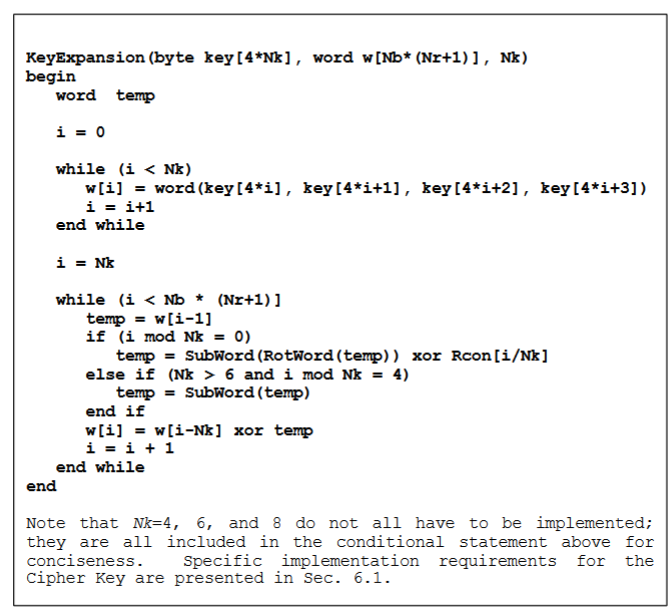
\includegraphics[width = 0.60\textwidth]{image8.png}
  \caption{Pseudoimplemetazione codice cifratura}
\end{figure}
\newpage

Viene allocato uno \textbf{scratchpad} di 2097152 bytes.\cite{crypto_note_standard_cryptonight}
Dall'output di Keccak vengono estratti i byte \texttt{64...191} e divisi
in 8 blocchi di 16 byte ciascuno. Ogni blocco viene cifrato utilizzando
il seguente codice:

\begin{algorithm}
  \caption{AES Rounds}
  \begin{algorithmic}[1]
  \For{$i = 0$ \textbf{to} $9$}
      \State block = \texttt{aes\_round}(block, round\_keys[$i$])
  \EndFor
  \end{algorithmic}
  \end{algorithm}


\subsubsection{Funzione cifratura AES}\label{funzione-cifratura-aes}

La funzione \texttt{aes\_round} esegue un round di cifratura AES, che
consiste nell'eseguire i passaggi seguenti sul blocco:

\begin{itemize}
\item
  SubBytes: ogni byte del blocco viene sostituito con un valore criptato
  utilizzando una tabella di sostituzione \emph{S-Box}.
\item
  ShiftRows: le righe del blocco vengono spostate di una posizione.
\item
  MixColumns: le colonne del blocco vengono mescolate utilizzando una
  matrice 4x4 nota come MDS, progettata per essere difficile
  da invertire.
\item
  Infine, il risultato è XORato con la chiave specifica per quel round.
  A differenza della classica funzione AES per cifrare, il primo e
  l'ultimo round quando si usano le \emph{round-keys} non sono speciali.
\end{itemize}

I blocchi che ne risultano vengono riportati nei primi 128 byte dello
scratchpad. Questi ultimi vengono cifrati nuovamente nello stesso modo,
e il risultato viene scritto nei successivi 128 byte. Questa operazione
viene effettuata 10 volte, per riempire tutto lo scratchpad di dati
pseudo-randomici. I byte \texttt{64..191}, che chiameremo
\emph{payload}, sono cifrati in questo modo 10 volte. 

\begin{figure}[h!]
  \centering
  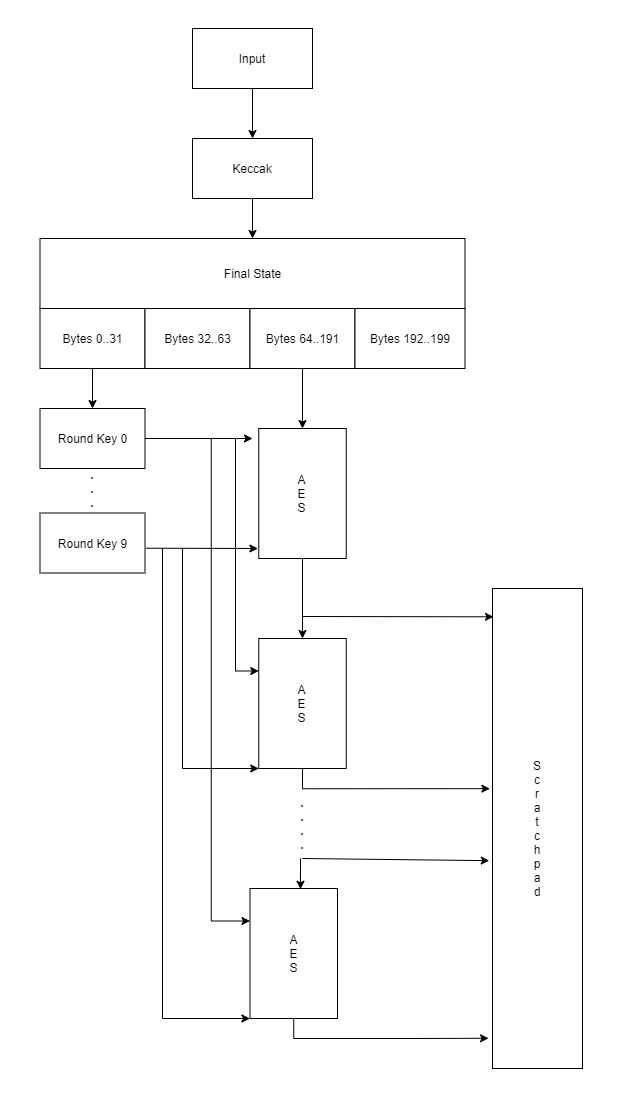
\includegraphics[width = 1\textwidth]{image_pt1.png}
  \caption{Diagramma inizializzazione scratchpad CryptoNight}
  \label{fig:my_label}
\end{figure}

\subsection{Seconda parte: Loop
memory-hard}\label{seconda-parte-loop-memory-hard}

La seconda parte si compone di un algoritmo che mantiene lo stato
composto da 52488 iterazioni. Si utilizzano operazioni
CPU-friendly, come la cifratura AES, XOR, moltiplicazioni e addizioni di
8 byte, per avere come unico

Prima di eseguire il loop utilizzato per rendere questa funzione di hash
\emph{memory-hard}, viene eseguito lo XOR sui byte \texttt{0..31} e i
byte \texttt{32..63} dell'output dell'hashing Keccak. I 32 byte
risultanti vengono utilizzati per inizializzare due variabili da 16 byte
ciascuna, \texttt{a} e \texttt{b}. Queste variabili vengono utilizzate
nel loop principale, composte da quattro passaggi:

\begin{enumerate}
\def\labelenumi{\arabic{enumi}.}
\item
  Il codice calcola l'indirizzo di memoria della variabile \texttt{a} e
  lo scrive sullo scratchpad. Per convertire un valore di 16 byte in un
  indirizzo nello scratchpad, bisogna interpretarlo come un intero
  rappresentato in little-endian, con gli ultimi 21 bit che
  rappresentano l'indice all'interno dei byte; gli ultimi 4 bit vengono
  comunque cancellati per ottenere l'allinamento a 16 byte, dato che i
  dati vengono letti e scritti sullo scratchpad in blocchi da 16 byte.
\item
  Successivamente, viene applicatata la funzione per cifrare il blocco
  \texttt{aes\_round} sull'indirizzo letto dallo scratchpad, con il
  valore di \texttt{a} usato come chiave.
\item
  Il risultato di questa operazione passa da uno XOR e il valore della
  variabile \texttt{b}, oltre ad essere scritto sullo scratchpad, sempre
  come indirizzo di memoria.
\item
  L'indirizzo ricavato viene letto dallo scratchpad e viene effettuata
  l'operazione di moltiplicazione chiamata \texttt{8byte\_mul}. Questa
  funzione, usa i primi 8 byte di ogni argomento, interpretati da essa
  come \texttt{uint\_64}, con rappresentazione little-endian. Il
  risultato di questa operazione viene convertito in 16 byte,
  concludendo l'operazione di moltiplicazione scambiando le due metà del
  risultato (8 byte ciascuna)
\item
  Il valore di \texttt{a} viene aggiunto, componente per componente in
  modulo 2\^{}64, al risultato della moltiplicazione con le due metà già
  scambiate attraverso la funzione \texttt{8byte\_add} che utilizza i
  primi 64 bit come intero senza segno, con il risultato che viene
  portato in 16 byte e scritto nello scratchpad.
\item
  Infine, viene letto l'indirizzo del risultato della cifratura
  dell'indirizzo della variabile di \texttt{a}, utilizzando come chiave
  \texttt{a} (il risultato del secondo passaggio) e viene effettuata un
  operazione di XOR con il risultato della addizione precedente.
\item
  Il risultato dell'operazione 6 viene utilizzato come nuovo valore
  della variabile \texttt{a}, mentre il risultato del passaggio 2 viene
  utilizzato come nuova variabile \texttt{b}.
\end{enumerate}



\begin{figure}[h!]
  \centering
  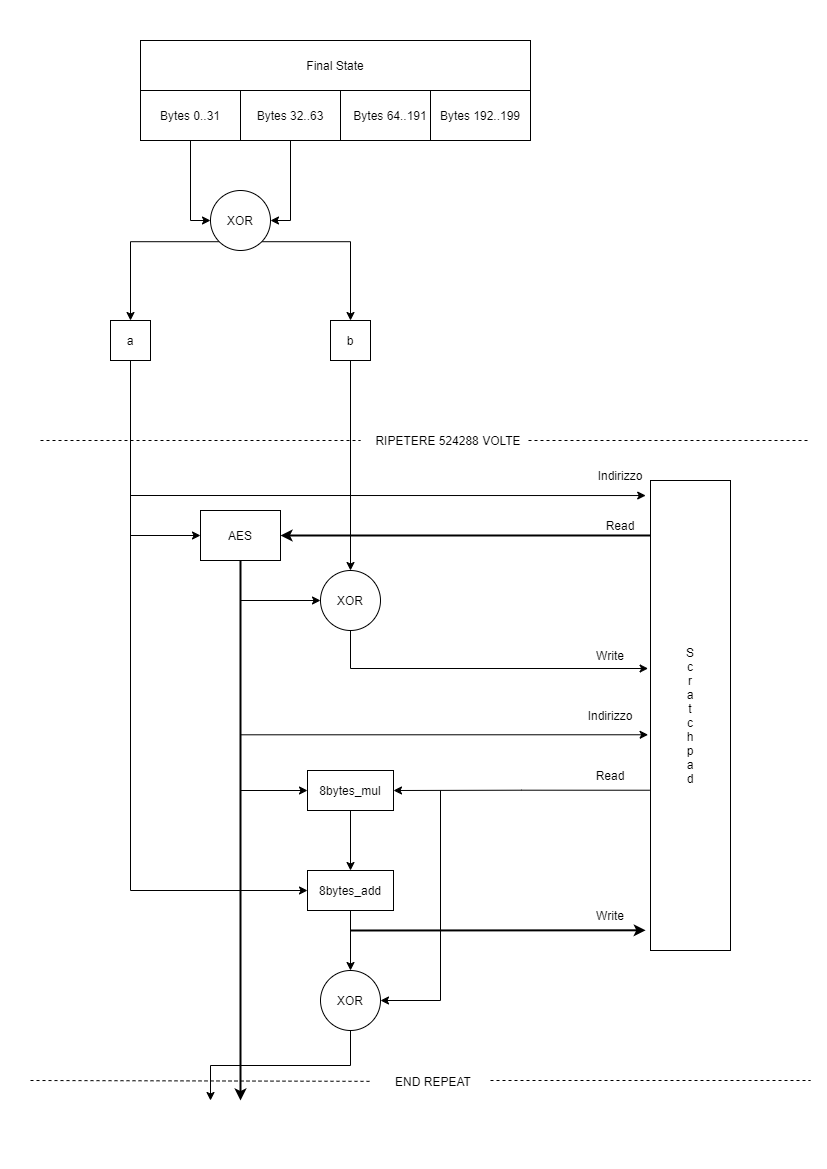
\includegraphics[width = 1\textwidth]{image_pt2.png}
  \caption{Diagramma loop memory-hard CryptoNight}
  \label{fig:my_label}
\end{figure}

\subsection{Terza parte: Calcolo del
risultato}\label{terza-parte-calcolo-del-risultato}

Dopo aver effettuato le operazioni memory-hard, i byte \texttt{32..63}
dati dall'hashing effettuato con Keccak vengono espansi in 10
\emph{round-keys} come nella prima parte.

I byte \texttt{64..191} dello stesso hashing vengono presi e viene
effettuato uno XOR con i primi 128 byte dello scratchpad. Il risultato
di questa operazione viene criptato con la funzione \texttt{aes\_round}
come nella prima parte, ma con le chiavi ricavate dall'espansione dei
byte \texttt{32..63}.\\
Il risultato di questa cifratura viene passato da uno XOR con i 128
bytes successivi dello scratchpad, cifrati nuovamente con la stessa
funzione, fino ad arrivare agli ultimi 128 byte dello scratchpad. Dopo
aver cifrato gli ultimi 128 byte viene effettuato lo XOR con gli ultimi
128 byte dello scratchpad.

I byte \texttt{64..191} del **Keccak state* vengono sostituiti con Il
risultato dell'operazione effettuata in precedenza. Tutti i 200 byte
dello stato di Keccak vengono passati da una permutazione, chiamata
\emph{Keccak-f}, con parametro \texttt{b\ =\ 1600}, l'implementazione
più sicura. Questa operazione viene effettuate per mescolare i bit dello
stato Keccak, in modo da rendere difficile la criptoanalisi del flusso
di dati.

Infine, i due bit più a destra vengono utilizzati per selezionare una
funzione di hash:

\begin{itemize}
  \item 
  0: BLAKE-256\cite{aumasson2008sha}
  \item
  1: Groest1-256\cite{groestl}
  \item 
  2: JH-256\cite{jh}
  \item 
  3: Skein-256\cite{skein}
\end{itemize}

L'output di questa funzione di hash viene applicato al Keccak state, e
l'hash risultante è l'output di CryptoNight. I diagrammi sottostanti rappresentano le operazioni
appena descritte graficamente.

\begin{figure}[h!]
  \centering
  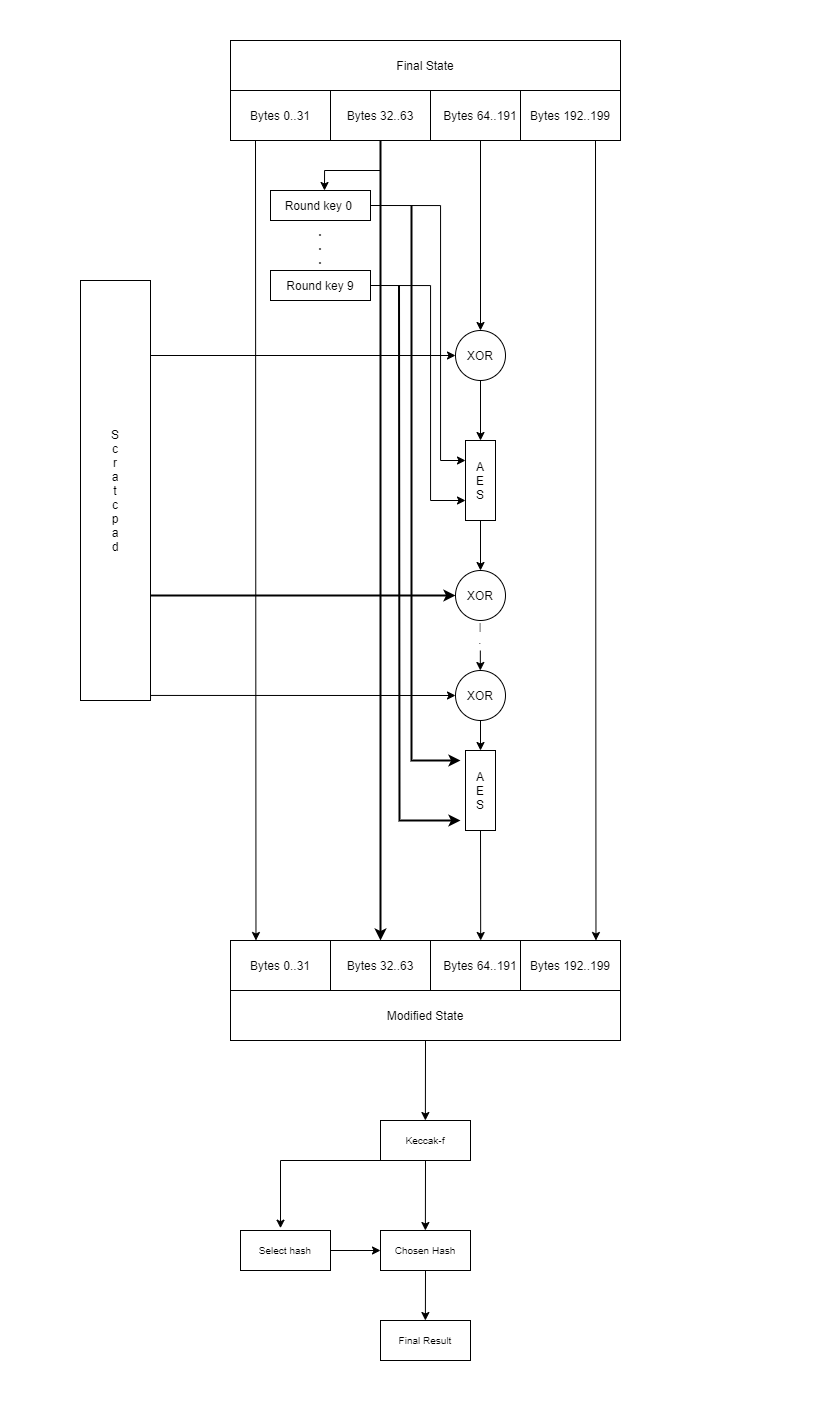
\includegraphics[width = 1\textwidth]{image_pt3.png}
  \caption{Diagramma calcolo del risultato dell'algoritmo CryptoNight}
  \label{fig:my_label}
\end{figure}
    % 3.2 da mergiare parte scritta con parte nuova
\section{Funzione di hash CryptoNight}\label{funzione-di-hash-cryptonight}

In questo capitolo parleremo del cuore del protocollo di consenso
CryptoNote, la funzione di hash \textbf{CryptoNight}, completa con le
sue specifiche e il suo funzionamento. L'obiettivo era il design di una
funzione che fosse facilmente eseguibile da CPU consumer-grade,
disponibili nei computer normali attraverso l'esecuzione di cifrature
AES, la moliplicazione di numeri a 64 bit e l'utilizzo di uno scratchpad
che, come da specifiche dell'algoritmo, entra nella dimensione di una
classica cache L3 di un processore dell'epoca (circa 2MB). La volontà,
più ambiziosa, era quella di rendere la funzione non facilmente
computabile dagli ASICs. Viene presentata come una funzione
\emph{memory-hard}, quindi resistente come algoritmo crittografico agli
attachi effettuati cercando di ridurre la complessità aumentando le
risorse hardware, progettata per essere inefficiente su GPU, FPGA e
ASICs rispetto alle classiche funzioni utilizzate nella
\emph{proof-of-work}, come ad esempio \emph{SHA-256}.

\subsubsection{Definizioni}\label{definizioni}

\begin{itemize}
\item
  Una \textbf{funzione di hash} è una funzione che trasforma dati di
  dimensione arbitraria in dati di dimensione fissata. L'operazione deve
  essere simile ad una funzione casuale per garantire la distribuzione
  uniforme dei risultati, indipendentemente dalla natura dei dati o
  dalle precedenti iterazioni dei dati.
\item
  \textbf{Scratchpad}: è una grande area di memoria temporanea e non
  persistente dove si possono eseguire calcoli senza alcuna conseguenza
  sullo stato a lungo termine.
\item
  \textbf{Memory-hard}: è una caratteristica delle funzioni di hash per
  il quale sono difficili da invertire, cioè trovare il dato originale a
  partire dal suo output, anche se si hanno risorse informatiche
  infinite.
\end{itemize}

\subsubsection{Primitive crittografiche
utilizzate}\label{primitive-crittografiche-utilizzate}

CryptoNight è basato su delle primitive crittografiche specifiche,
composte da 
\begin{itemize}
  \item
  Cifratura AES a 256bit
  \item 5 funzioni di hash, finaliste
  nella competizione per la ricerca di un nuovo standard per le funzioni
  di hash del 2012 condotto dal NIST:
  \begin{itemize}
    \item Keccak
    \item BLAKE
    \item Groest1
    \item JH
    \item Skein
  \end{itemize}
\end{itemize}

\subsection{Prima parte: Inizializzazione dello
scratchpad}\label{prima-parte-inizializzazione-dello-scratchpad}

L'input della funzione di hash (in Monero, ad esempio, di dimensione 80
bytes) viene passato nella funzione di hash di Keccak\cite{bertoni2011keccak}. Viene scelta con
\texttt{b\ =\ 1600}, quindi con dimensione dell'output di 1600 bit o 200
bytes e con dimensione del digest di 512 bits o 64 bytes con il
parametro \texttt{c\ =\ 512}. Questi byte saranno definiti come
\textbf{Keccak state} \cite{keccak_parameters}

I byte \texttt{0..31} risultanti dall'output della funzione vengono
scelti come chiave per l'algoritmo di cifratura AES-256. La chiave non
viene utilizzata così com'è, ma viene espansa\cite{standard2001federal} in 10 sotto-chiavi, con lo
scopo di rendere l'algoritmo più sicuro, utilizzando più di una chiave
AES per cifrare. L'espansione viene fatta dividendo la chiave in 8
parole di 4 byte ciascuna. Per generare le due parole rimaste al fine
completare i 10 \emph{key rounds} , si esegue la rotazione
dell'ultima parola generata, effettuata con la funzione
\texttt{RotWord()}, che esegue una permutazione ciclica e avendo come
input {[}\emph{a0,a1,a2,a3}{]} ritorna {[}\emph{a1,a2,a3,a4}{]}.
Successivamente vengono sostituiti i byte utilizzando una \textbf{S-Box}
e viene eseguito uno XOR con una costante chiamata \texttt{Rcon} (Round
constant). I dettagli di una pseudo implementazione del codice per
l'espansione della chiave è presente qui.

\begin{figure}
  \centering
  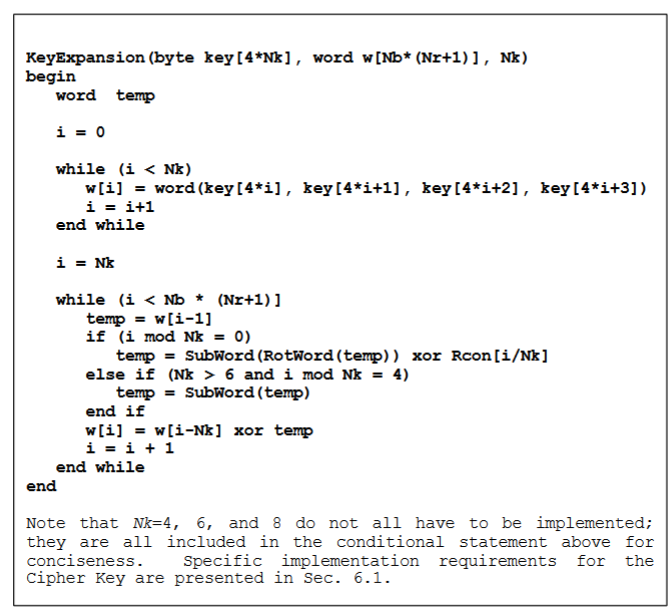
\includegraphics[width = 0.60\textwidth]{image8.png}
  \caption{Pseudoimplemetazione codice cifratura}
\end{figure}
\newpage

Viene allocato uno \textbf{scratchpad} di 2097152 bytes.\cite{crypto_note_standard_cryptonight}
Dall'output di Keccak vengono estratti i byte \texttt{64...191} e divisi
in 8 blocchi di 16 byte ciascuno. Ogni blocco viene cifrato utilizzando
il seguente codice:

\begin{algorithm}
  \caption{AES Rounds}
  \begin{algorithmic}[1]
  \For{$i = 0$ \textbf{to} $9$}
      \State block = \texttt{aes\_round}(block, round\_keys[$i$])
  \EndFor
  \end{algorithmic}
  \end{algorithm}


\subsubsection{Funzione cifratura AES}\label{funzione-cifratura-aes}

La funzione \texttt{aes\_round} esegue un round di cifratura AES, che
consiste nell'eseguire i passaggi seguenti sul blocco:

\begin{itemize}
\item
  SubBytes: ogni byte del blocco viene sostituito con un valore criptato
  utilizzando una tabella di sostituzione \emph{S-Box}.
\item
  ShiftRows: le righe del blocco vengono spostate di una posizione.
\item
  MixColumns: le colonne del blocco vengono mescolate utilizzando una
  matrice 4x4 nota come MDS, progettata per essere difficile
  da invertire.
\item
  Infine, il risultato è XORato con la chiave specifica per quel round.
  A differenza della classica funzione AES per cifrare, il primo e
  l'ultimo round quando si usano le \emph{round-keys} non sono speciali.
\end{itemize}

I blocchi che ne risultano vengono riportati nei primi 128 byte dello
scratchpad. Questi ultimi vengono cifrati nuovamente nello stesso modo,
e il risultato viene scritto nei successivi 128 byte. Questa operazione
viene effettuata 10 volte, per riempire tutto lo scratchpad di dati
pseudo-randomici. I byte \texttt{64..191}, che chiameremo
\emph{payload}, sono cifrati in questo modo 10 volte. 

\begin{figure}[h]
  \centering
  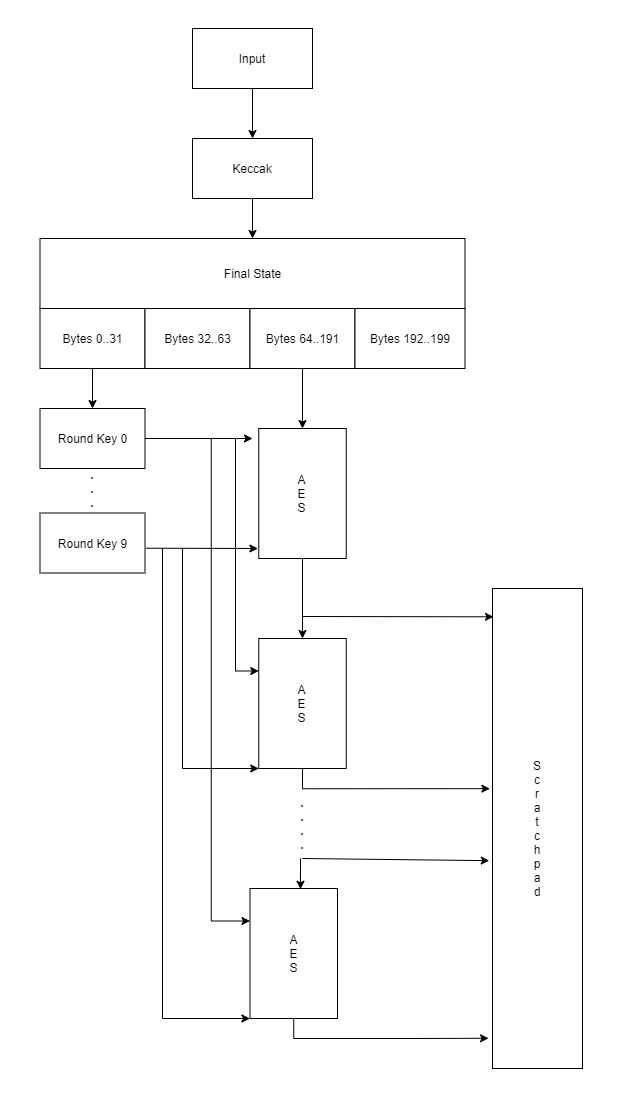
\includegraphics[width = 1\textwidth]{image_pt1.png}
  \caption{Diagramma inizializzazione scratchpad CryptoNight}
  \label{fig:my_label}
\end{figure}

\subsection{Seconda parte: Loop
memory-hard}\label{seconda-parte-loop-memory-hard}

La seconda parte si compone di un algoritmo che mantiene lo stato
composto da 52488 iterazioni. Si utilizzano operazioni
CPU-friendly, come la cifratura AES, XOR, moltiplicazioni e addizioni di
8 byte, per avere come unico

Prima di eseguire il loop utilizzato per rendere questa funzione di hash
\emph{memory-hard}, viene eseguito lo XOR sui byte \texttt{0..31} e i
byte \texttt{32..63} dell'output dell'hashing Keccak. I 32 byte
risultanti vengono utilizzati per inizializzare due variabili da 16 byte
ciascuna, \texttt{a} e \texttt{b}. Queste variabili vengono utilizzate
nel loop principale, composte da quattro passaggi:

\begin{enumerate}
\def\labelenumi{\arabic{enumi}.}
\item
  Il codice calcola l'indirizzo di memoria della variabile \texttt{a} e
  lo scrive sullo scratchpad. Per convertire un valore di 16 byte in un
  indirizzo nello scratchpad, bisogna interpretarlo come un intero
  rappresentato in little-endian, con gli ultimi 21 bit che
  rappresentano l'indice all'interno dei byte; gli ultimi 4 bit vengono
  comunque cancellati per ottenere l'allinamento a 16 byte, dato che i
  dati vengono letti e scritti sullo scratchpad in blocchi da 16 byte.
\item
  Successivamente, viene applicatata la funzione per cifrare il blocco
  \texttt{aes\_round} sull'indirizzo letto dallo scratchpad, con il
  valore di \texttt{a} usato come chiave.
\item
  Il risultato di questa operazione passa da uno XOR e il valore della
  variabile \texttt{b}, oltre ad essere scritto sullo scratchpad, sempre
  come indirizzo di memoria.
\item
  L'indirizzo ricavato viene letto dallo scratchpad e viene effettuata
  l'operazione di moltiplicazione chiamata \texttt{8byte\_mul}. Questa
  funzione, usa i primi 8 byte di ogni argomento, interpretati da essa
  come \texttt{uint\_64}, con rappresentazione little-endian. Il
  risultato di questa operazione viene convertito in 16 byte,
  concludendo l'operazione di moltiplicazione scambiando le due metà del
  risultato (8 byte ciascuna)
\item
  Il valore di \texttt{a} viene aggiunto, componente per componente in
  modulo 2\^{}64, al risultato della moltiplicazione con le due metà già
  scambiate attraverso la funzione \texttt{8byte\_add} che utilizza i
  primi 64 bit come intero senza segno, con il risultato che viene
  portato in 16 byte e scritto nello scratchpad.
\item
  Infine, viene letto l'indirizzo del risultato della cifratura
  dell'indirizzo della variabile di \texttt{a}, utilizzando come chiave
  \texttt{a} (il risultato del secondo passaggio) e viene effettuata un
  operazione di XOR con il risultato della addizione precedente.
\item
  Il risultato dell'operazione 6 viene utilizzato come nuovo valore
  della variabile \texttt{a}, mentre il risultato del passaggio 2 viene
  utilizzato come nuova variabile \texttt{b}.
\end{enumerate}



\begin{figure}[h]
  \centering
  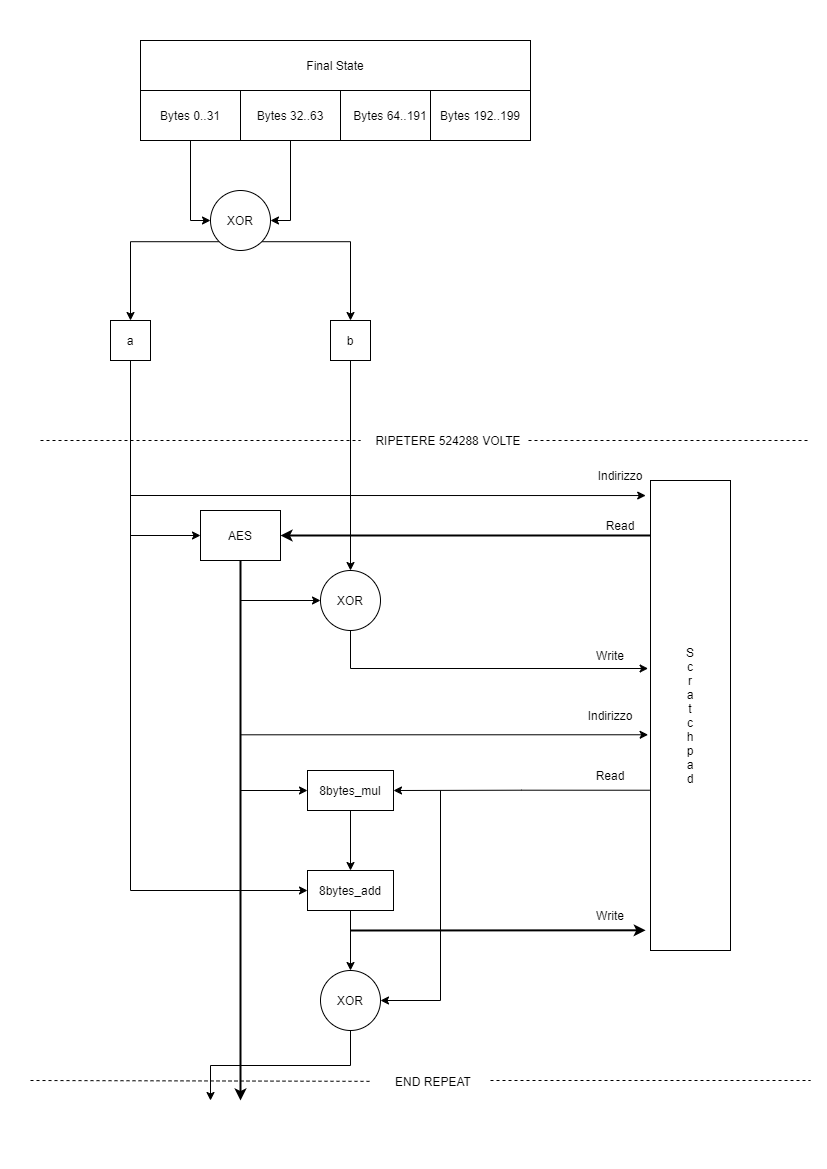
\includegraphics[width = 1\textwidth]{image_pt2.png}
  \caption{Diagramma loop memory-hard CryptoNight}
  \label{fig:my_label}
\end{figure}

\subsection{Terza parte: Calcolo del
risultato}\label{terza-parte-calcolo-del-risultato}

Dopo aver effettuato le operazioni memory-hard, i byte \texttt{32..63}
dati dall'hashing effettuato con Keccak vengono espansi in 10
\emph{round-keys} come nella prima parte.

I byte \texttt{64..191} dello stesso hashing vengono presi e viene
effettuato uno XOR con i primi 128 byte dello scratchpad. Il risultato
di questa operazione viene criptato con la funzione \texttt{aes\_round}
come nella prima parte, ma con le chiavi ricavate dall'espansione dei
byte \texttt{32..63}.\\
Il risultato di questa cifratura viene passato da uno XOR con i 128
bytes successivi dello scratchpad, cifrati nuovamente con la stessa
funzione, fino ad arrivare agli ultimi 128 byte dello scratchpad. Dopo
aver cifrato gli ultimi 128 byte viene effettuato lo XOR con gli ultimi
128 byte dello scratchpad.

I byte \texttt{64..191} del **Keccak state* vengono sostituiti con Il
risultato dell'operazione effettuata in precedenza. Tutti i 200 byte
dello stato di Keccak vengono passati da una permutazione, chiamata
\emph{Keccak-f}, con parametro \texttt{b\ =\ 1600}, l'implementazione
più sicura. Questa operazione viene effettuate per mescolare i bit dello
stato Keccak, in modo da rendere difficile la criptoanalisi del flusso
di dati.

Infine, i due bit più a destra vengono utilizzati per selezionare una
funzione di hash:

\begin{itemize}
  \item 
  0: BLAKE-256\cite{aumasson2008sha}
  \item
  1: Groest1-256\cite{groestl}
  \item 
  2: JH-256\cite{jh}
  \item 
  3: Skein-256\cite{skein}
\end{itemize}

L'output di questa funzione di hash viene applicato al Keccak state, e
l'hash risultante è l'output di CryptoNight. I diagrammi sottostanti rappresentano le operazioni
appena descritte graficamente.

\begin{figure}[h]
  \centering
  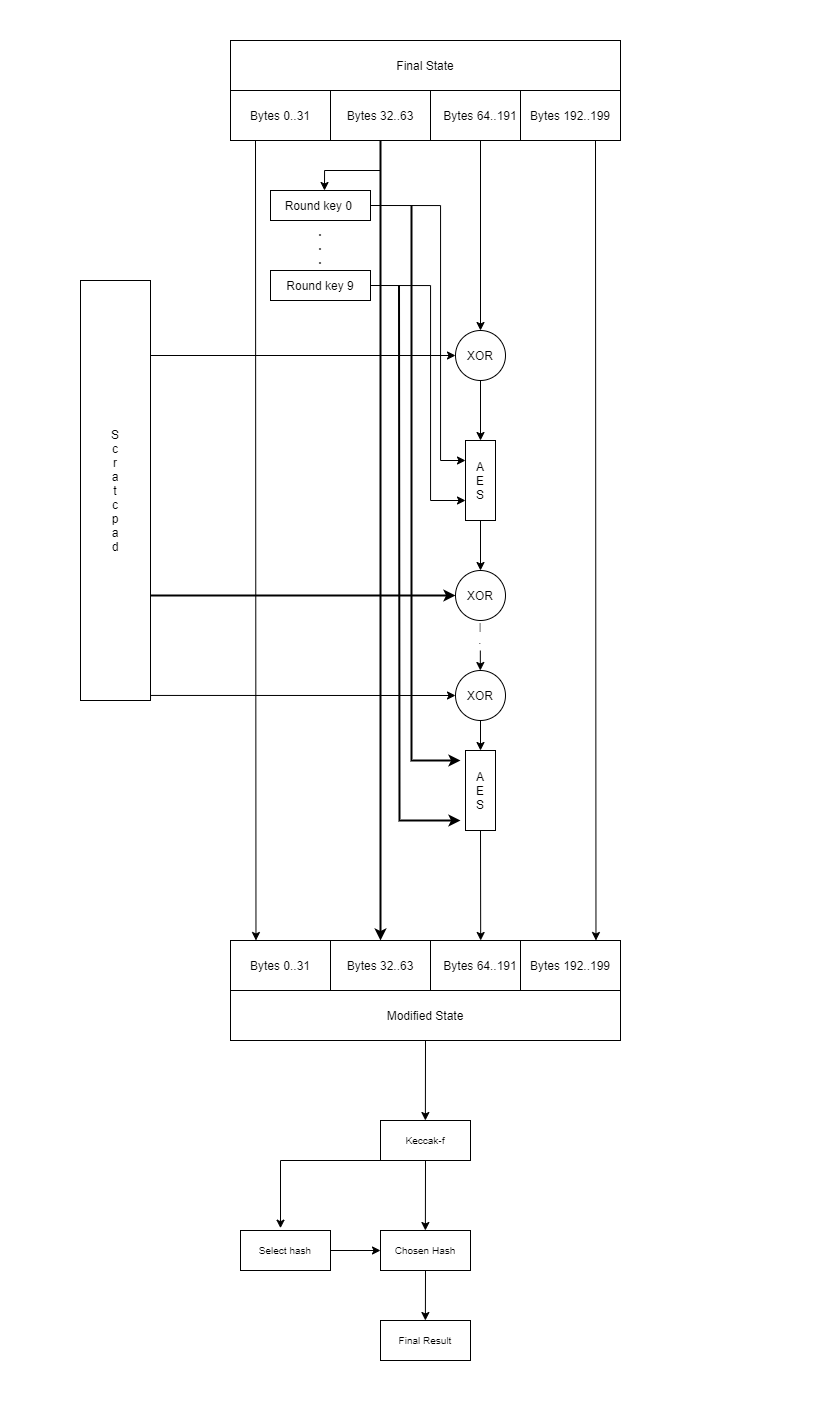
\includegraphics[width = 1\textwidth]{image_pt3.png}
  \caption{Diagramma calcolo del risultato dell'algoritmo CryptoNight}
  \label{fig:my_label}
\end{figure} % TODO stesso discorso della prima. non è un nuovo chapter e attualmente secondo me così ci sta.

\chapter{RandomX}
Il seguente capitolo entra nel dettaglio dell'implementazione del successore di CryptoNight, denominato RandomX. CryptoNight è diventato obsoleto poiché non più resistente agli ASIC. Di conseguenza, RandomX è stato sviluppato esternamente a CryptoNote, ma dato che è attualmente l'ultima versione degli algoritmi PoW ASIC-resistant, si è deciso di includerlo. 
Tutte le informazioni, presentate in questo capitolo, sono state reperite dalla pagina GitHub ufficiale \cite{randomx}.

\section{Design di Randomx}
Per minimizzare il vantaggio di hardware specializzati come gli ASIC, già discussi in precedenza, un algoritmo di \textbf{Proof of Work} (\textbf{PoW}) deve potersi legare ai dispositivi esistenti il cui uso risulti essere ampiamente diffuso. Non a caso, si focalizza sull'utilizzo delle \textbf{CPU} per i seguenti motivi:

\begin{itemize}
    \item \textbf{Accessibilità}: Le CPU, essendo meno specializzate, sono più diffuse e accessibili. Un algoritmo basato su CPU è più \textbf{egalitario} e permette a più partecipanti di unirsi alla rete, contrariamente a ciò che accadeva con gli ASIC in quanto il loro notevole costo permetteva una centralizzazione del mining nelle mani di pochi;
    \item \textbf{Istruzioni Hardware Comuni}: CPU diverse \textbf{condividono} un grande \textit{subset} di istruzioni hardware native;
    \item \textbf{Documentazione e Compilatori}: Tutti i principali set di istruzioni CPU sono ben \textbf{documentati} con diversi compilatori \textbf{open-source} disponibili.
\end{itemize}

\subsection{Prova di Lavoro Dinamica} 
L'idea alla base di una \textbf{Proof of Work} basata su CPU è l'impiego di un \textit{lavoro dinamico} sfruttando il fatto che queste accettano come input non solo \textbf{dati}, come le tipiche funzioni di hash crittografiche, ma anche il \textbf{codice}. Ciò evita che le sequenza delle operazioni sia fissa e quindi più facilmente eseguibile da un circuito integrato specializzato. Una \textbf{Proof of Work dinamica} consiste in 4 steps:
\begin{enumerate}
    \item Generazione di un programma casuale;
    \item Traduzione in codice macchina nativo della CPU;
    \item Esecuzione del programma;
    \item Trasformazione dell'output del programma in un valore crittograficamente sicuro.
\end{enumerate}

\subsubsection{Generazione di un programma casuale}
Inizialmente la progettazione di una Proof of Work si basava sulla generazione di un programma in linguaggi ad alto livello, come C o Javascript, ma questi per via della loro sintassi complessa, implicavano notevoli costi in termini di tempo.

Il modo più veloce per generare un programma casuale è utilizzare un generatore senza logica, riempiendo semplicemente un \textbf{buffer con dati casuali}. Questo richiede la progettazione di un linguaggio di programmazione senza sintassi, in cui tutte le stringhe di bit casuali rappresentano programmi validi.

\subsubsection{Traduzione del Programma in Codice Macchina}
Per generare il codice macchina il più velocemente possibile, il nostro set di istruzioni deve essere il più vicino possibile all'hardware nativo, ma allo stesso tempo deve risultare abbastanza generico in modo da non limitare l'algoritmo a una specifica architettura CPU.

\subsubsection{Esecuzione del Programma}
L'esecuzione del programma dovrebbe utilizzare il \textbf{maggior numero} possibile di \textbf{componenti della CPU}. Alcune delle caratteristiche che dovrebbero essere sfruttate sono:
\begin{itemize}
    \item Cache multi-livello (L1, L2, L3);
    \item Cache  \textmu op;
    \item Unità logica aritmetica (ALU);
    \item Unità a virgola mobile (FPU);
    \item Controller di memoria;
    \item Parallelismo a livello di istruzione;
    \item Esecuzione fuori ordine;
    \item Esecuzione speculativa;
    \item Rinominazione dei registri.
\end{itemize}

\subsubsection{Calcolo del Risultato Finale}
\textbf{Blake2b} è una funzione di hashing crittograficamente sicura, progettata per essere veloce nel software, soprattutto sui moderni processori a 64 bit, dove è circa tre volte più veloce di SHA-3. Proprio per questo è ideale per essere utilizzata in una \textbf{Proof of Work} basata su \textbf{CPU}.

Per quanto riguarda, invece, l'elaborazione di grandi quantità di dati in modo crittograficamente sicuro, l'\textbf{Advanced Encryption Standard }(\textbf{AES}) può fornire la massima velocità di elaborazione perché molte CPU moderne supportano l'accelerazione hardware di queste operazioni.

\subsection{"Easy program problem"}
Il problema dell'\textit{easy program} si basa sul fatto che quando viene generato un programma casuale, si potrebbe decidere di eseguirlo solo in caso sia favorevole. Questa strategia è fattibile per due motivi principali:

\begin{itemize}
    \item \textbf{Distribuzione del Tempo di Esecuzione}: I tempi di esecuzione dei programmi generati casualmente seguono tipicamente una \textit{distribuzione log-normale}. Questi possono rapidamente analizzati e in caso di tempo di esecuzione superiore alla media, l'esecuzione può essere saltata e può essere generato un nuovo programma. Se quest'ultima operazione risulta essere economica, può migliorare significativamente le prestazioni.
    \item \textbf{Ottimizzazione delle Caratteristiche}: Un'implementazione potrebbe scegliere di ottimizzare un sottoinsieme delle caratteristiche necessarie per l'esecuzione del programma. Ad esempio, si può decidere di eliminare il supporto per alcune operazioni (come la divisione) o di implementare alcune sequenze di istruzioni in modo più efficiente. In seguito, i programmi generati verrebbero analizzati ed eseguiti solo se soddisfano i requisiti specifici dell'implementazione ottimizzata.
\end{itemize}

Queste strategie di ricerca di programmi con particolari proprietà vanno in \textbf{contrasto} con gli obiettivi di questa \textbf{Proof of Work}, quindi devono essere eliminate:
\begin{itemize}
    \item \textbf{Soluzione}: Esecuzione di una sequenza di \textbf{N programmi casuali}, in modo che ogni programma sia generato dall'\textbf{output del precedente}. L'output del programma finale viene quindi utilizzato come risultato.
    \item \textbf{Principio}: Una volta eseguito il primo programma, un miner deve decidere \textbf{se impegnarsi a terminare l'intera catena} (che può includere programmi sfavorevoli) o ricominciare da capo e sprecare lo sforzo impiegato sulla catena non completata;
    \item \textbf{Vantaggio}: Uniformare il tempo di esecuzione per l'intera catena, poiché la deviazione relativa di una somma di tempi di esecuzione distribuiti identicamente è ridotta.
\end{itemize}

\subsection{Tempo di verifica}
Poiché lo scopo del \textbf{Proof of Work} è di essere utilizzato in una \textbf{rete peer-to-peer} senza fiducia, i partecipanti alla rete devono essere in grado di verificare rapidamente se una prova è valida o meno. Ciò pone un \textbf{limite} superiore alla \textbf{complessità dell'algoritmo} di \textbf{Proof of Work}. In particolare, abbiamo fissato l'obiettivo per RandomX di essere almeno altrettanto veloce da verificare quanto la funzione di hash CryptoNight, che mira a sostituire.

\subsection{Memory-hardness}
Oltre alle risorse computazionali pure, come \textbf{ALU} e \textbf{FPU}, le \textbf{CPU} di solito hanno accesso a una grande quantità di memoria sotto forma di DRAM. Le prestazioni del sottosistema di memoria sono tipicamente ottimizzate per adattarsi alle capacità di calcolo.

Per utilizzare la \textbf{memoria esterna} così come i controller di memoria on-chip, l'\textbf{algoritmo di Proof of Work} dovrebbe accedere a un grande \textbf{buffer} di memoria (chiamato "\textbf{Dataset}"). Il Dataset deve essere:

\begin{itemize}
    \item \textbf{più grande} di quanto possa essere memorizzato on-chip (per richiedere memoria esterna);
    \item \textbf{dinamico} (per richiedere memoria scrivibile)
\end{itemize}

Idealmente, la dimensione del Dataset dovrebbe essere di almeno 4 GiB. Tuttavia, a causa dei vincoli sul tempo di verifica la dimensione utilizzata da RandomX è stata selezionata a 2080 MiB.

\section{Architettura della macchina virtuale}

Questa sezione descrive la progettazione della macchina virtuale (VM) di RandomX.

\subsection{Set di istruzioni}

RandomX utilizza una codifica delle istruzioni a lunghezza fissa con 8 byte per istruzione. Questo permette di includere un valore immediato a 32 bit nella parola dell'istruzione.

\subsection{Programma}

Il programma eseguito dalla VM ha la forma di un loop composto da 256 istruzioni casuali.

\begin{itemize}
  \item 256 istruzioni sono sufficientemente lunghe da fornire un gran numero di programmi possibili e abbastanza spazio per i branch. Il numero di programmi diversi che possono essere generati è limitato a $2^{512} = 1.3 \times 10^{154}$, che è il numero di valori di seme possibili del generatore casuale.
  \item 256 istruzioni sono abbastanza brevi affinché le CPU ad alte prestazioni possano eseguire una iterazione in un tempo simile a quello necessario per recuperare i dati dalla DRAM. Questo è vantaggioso perché permette di sincronizzare e prefetchare completamente gli accessi al Dataset (vedi capitolo 2.9).
  \item Poiché il programma è un loop, può sfruttare la $\mu$op cache che è presente in alcune CPU x86. Eseguire un loop dalla $\mu$op cache permette alla CPU di spegnere i decoder delle istruzioni x86, il che dovrebbe aiutare a equilibrare l'efficienza energetica tra x86 e architetture con decodifica delle istruzioni semplice.
\end{itemize}

\subsection{Registri}

La VM utilizza 8 registri interi e 12 registri floating-point. Questo è il massimo che può essere allocato come registri fisici in x86-64, che ha il minor numero di registri architetturali tra le comuni architetture CPU a 64 bit. Utilizzare più registri metterebbe le CPU x86 in svantaggio poiché dovrebbero utilizzare la memoria per memorizzare i contenuti dei registri della VM.

\subsection{Operazioni intere}

RandomX utilizza tutte le operazioni intere primitive che hanno un'elevata entropia di output: addizione (IADD\_RS, IADD\_M), sottrazione (ISUB\_R, ISUB\_M, INEG\_R), moltiplicazione (IMUL\_R, IMUL\_M, IMULH\_R, IMULH\_M, ISMULH\_R, ISMULH\_M, IMUL\_RCP), exclusive or (IXOR\_R, IXOR\_M) e rotazione (IROR\_R, IROL\_R).

\subsection{Operazioni floating-point}

RandomX utilizza operazioni floating-point (virgola mobile) a doppia precisione, che sono supportate dalla maggior parte delle CPU e richiedono hardware più complesso rispetto alla singola precisione. Tutte le operazioni vengono eseguite come operazioni vettoriali a 128 bit, anch'esse supportate da tutte le principali architetture CPU.

RandomX utilizza cinque operazioni garantite dallo standard IEEE 754 per dare risultati arrotondati correttamente: addizione, sottrazione, moltiplicazione, divisione e radice quadrata. Tutte le 4 modalità di arrotondamento definite dallo standard vengono utilizzate.

\subsection{Branch}

Le CPU moderne investono molta area del die e energia per gestire i branch. Questo include:

\begin{itemize}
  \item Branch predictor unit
  \item Stati di checkpoint/rollback che permettono alla CPU di recuperare in caso di una predizione errata del branch.
\end{itemize}

Per sfruttare i progetti speculativi, i programmi casuali dovrebbero contenere branch. Tuttavia, se la predizione dei branch fallisce, le istruzioni eseguite speculativamente vengono scartate, il che comporta una certa quantità di energia sprecata con ogni predizione errata. Pertanto dovremmo mirare a minimizzare il numero di predizioni errate.

Inoltre, i branch nel codice sono essenziali perché riducono significativamente il numero di ottimizzazioni statiche che possono essere effettuate. Ad esempio, considera la seguente sequenza di istruzioni x86:
\begin{verbatim}
    ...
branch_target_00:
    ...
    xor r8, r9
    test r10, 2088960
    je branch_target_00
    xor r8, r9
    ...
\end{verbatim}
Le operazioni XOR normalmente si annullerebbero, ma non possono essere ottimizzate via a causa del branch perché il risultato sarà diverso se il branch viene preso. Analogamente, l'istruzione ISWAP\_R potrebbe essere sempre ottimizzata staticamente se non fosse per i branch.

In generale, i branch casuali devono essere progettati in modo tale che:

1. Non siano possibili loop infiniti.
2. Il numero di branch predetti erroneamente sia piccolo.
3. La condizione del branch dipenda da un valore a runtime per disabilitare le ottimizzazioni statiche del branch.

\subsection{Parallelismo a livello di istruzione}

Le CPU migliorano le loro prestazioni utilizzando diverse tecniche che sfruttano il parallelismo a livello di istruzione del codice eseguito. Queste tecniche includono:

\begin{itemize}
  \item Avere più unità di esecuzione che possono eseguire operazioni in parallelo (\textit{superscalar execution}).
  \item Eseguire istruzioni non nell'ordine del programma, ma nell'ordine della disponibilità degli operandi (\textit{out-of-order execution}).
  \item Prevedere quale direzione prenderanno i branch per migliorare i benefici sia dell'esecuzione superscalare che di quella out-of-order.
\end{itemize}

RandomX beneficia di tutte queste ottimizzazioni.

\subsection{Scratchpad}

Lo Scratchpad è una "zona di lavoro" utilizzata come memoria di lettura-scrittura. La sua dimensione è stata selezionata per adattarsi completamente nella cache della CPU.

\subsection{Dataset}

Poiché lo Scratchpad viene solitamente memorizzato nella cache della CPU, solo gli accessi al Dataset utilizzano i controller di memoria.

RandomX legge casualmente dal Dataset una volta per iterazione del programma (16384 volte per risultato hash). Poiché il Dataset deve essere memorizzato nella DRAM, fornisce un limite naturale alla parallelizzazione, poiché la DRAM non può effettuare più di circa 25 milioni di accessi casuali al secondo per gruppo di banchi. Ogni gruppo di banchi indirizzabili separatamente consente un throughput di circa 1500 H/s.

Tutti gli accessi al Dataset leggono una linea di cache della CPU (64 byte) e sono completamente prefetchati. Il tempo per eseguire una iterazione del programma descritta nel capitolo 4.6.2 della Specifica è circa lo stesso della latenza tipica di accesso alla DRAM (50-100 ns).

\section{Funzioni personalizzate}

\subsection{AesGenerator1R}

\texttt{AesGenerator1R} è stato progettato per la generazione più veloce possibile di dati pseudocasuali per riempire lo Scratchpad. Sfrutta l'AES accelerato via hardware nelle CPU moderne. Viene eseguito solo un round AES per ogni 16 byte di output, il che si traduce in un throughput superiore a 20 GB/s nella maggior parte delle CPU moderne.

AesGenerator1R fornisce una buona distribuzione dell'output a condizione che venga inizializzato con uno stato iniziale sufficientemente 'casuale' (vedi Appendice F).

\subsection{AesGenerator4R}

\texttt{AesGenerator4R} utilizza 4 round AES per generare dati pseudocasuali per l'inizializzazione del Program Buffer. Poiché 2 round AES sono sufficienti per l'effetto valanga completo di tutti i bit di input, AesGenerator4R ha eccellenti proprietà statistiche (vedi Appendice F) mantenendo comunque prestazioni molto buone.

La natura reversibile di questo generatore non è un problema poiché lo stato del generatore viene sempre inizializzato utilizzando l'output di una funzione di hash non reversibile (Blake2b).

\subsection{AesHash1R}

\texttt{AesHash} è stato progettato per il calcolo più veloce possibile dell'impronta digitale dello Scratchpad. Interpreta lo Scratchpad come un insieme di chiavi di round AES, quindi è equivalente alla crittografia AES con 32768 round. Vengono eseguiti due round extra alla fine per garantire l'effetto valanga di tutti i bit dello Scratchpad in ogni lane.

La natura reversibile di AesHash1R non è un problema per due motivi principali:

\begin{itemize}
  \item Non è possibile controllare direttamente l'input di AesHash1R.
  \item L'output di AesHash1R viene passato alla funzione di hash Blake2b, che non è reversibile.
\end{itemize}

\subsection{SuperscalarHash}

\texttt{SuperscalarHash} è stato progettato per consumare quanta più energia possibile mentre la CPU attende che i dati vengano caricati dalla DRAM. La latenza target di 170 cicli corrisponde alla latenza usuale della DRAM di 40-80 ns e alla frequenza di clock di 2-4 GHz. I dispositivi ASIC progettati per il mining in modalità leggera con memoria a bassa latenza saranno limitati da SuperscalarHash durante il calcolo degli elementi del Dataset e la loro efficienza sarà compromessa dall'alto consumo energetico di SuperscalarHash.

La funzione SuperscalarHash media contiene un totale di 450 istruzioni, di cui 155 sono moltiplicazioni a 64 bit. In media, la catena di dipendenze più lunga è composta da 95 istruzioni. Un progetto ASIC per il mining in modalità leggera, con 256 MiB di memoria on-die e una latenza di 1 ciclo per tutte le operazioni, avrà bisogno in media di 95 * 8 = 760 cicli per costruire un elemento del Dataset, assumendo una parallelizzazione illimitata. Dovrà eseguire 155 * 8 = 1240 moltiplicazioni a 64 bit per elemento, il che consumerà energia comparabile al caricamento di 64 byte dalla DRAM.



\section{Descrizione dell'algoritmo}

L'algoritmo RandomX accetta due valori di input e produce un risultato di 256 bit \texttt{R}.
I due input consiston in: 

\begin{itemize}
    \item Una stringa \texttt{K} di dimensione 0-60 byte (chiave)
    \item Una stringa \texttt{H} di lunghezza arbitraria (valore da hashare)
\end{itemize}

\noindent
L'algoritmo consiste nei seguenti passaggi:

\begin{enumerate}
    \item Il Dataset viene inizializzato utilizzando il valore della chiave \texttt{K}.
    \item Il seed di 64 byte \texttt{S} viene calcolato come \texttt{S = Hash512(H)}.
    \item Sia \texttt{gen1 = AesGenerator1R(S)}.
    \item Lo Scratchpad viene riempito con \texttt{RANDOMX\_SCRATCHPAD\_L3} byte casuali utilizzando il generatore \texttt{gen1}.
    \item Sia \texttt{gen4 = AesGenerator4R(gen1.state)} (usare lo stato finale di \texttt{gen1}).
    \item Il valore del registro della VM \texttt{fprc} è impostato a 0 (modalità di arrotondamento predefinita).
    \item La VM viene programmata utilizzando \texttt{128 + 8 * RANDOMX\_PROGRAM\_SIZE} byte casuali utilizzando il generatore \texttt{gen4}.
    \item La VM viene eseguita.
    \item Un nuovo seed di 64 byte viene calcolato come \texttt{S = Hash512(RegisterFile)}.
    \item Imposta \texttt{gen4.state = S} (modifica lo stato del generatore).
    \item I passaggi 7-10 vengono eseguiti un totale di \texttt{RANDOMX\_PROGRAM\_COUNT} volte. L'ultima iterazione salta i passaggi 9 e 10.
    \item L'impronta digitale dello Scratchpad viene calcolata come \texttt{A = AesHash1R(Scratchpad)}.
    \item I byte 192-255 del Registro File vengono impostati al valore di \texttt{A}.
    \item Il risultato viene calcolato come \texttt{R = Hash256(RegisterFile)}. 
    \\
\end{enumerate}

\noindent
L'input della funzione \texttt{Hash512} nel passaggio 9 è il seguente:

\begin{verbatim}
 +---------------------------------+
 |         registri r0-r7          | (64 byte)
 +---------------------------------+
 |         registri f0-f3          | (64 byte)
 +---------------------------------+
 |         registri e0-e3          | (64 byte)
 +---------------------------------+
 |         registri a0-a3          | (64 byte)
 +---------------------------------+
\end{verbatim}

\noindent
Invece, l'input della funzione \texttt{Hash256} nel passaggio 14 è il seguente:

\begin{verbatim}
 +---------------------------------+
 |         registri r0-r7          | (64 byte)
 +---------------------------------+
 |         registri f0-f3          | (64 byte)
 +---------------------------------+
 |         registri e0-e3          | (64 byte)
 +---------------------------------+
 |      AesHash1R(Scratchpad)      | (64 byte)
 +---------------------------------+
\end{verbatim}


% TODO
% aggiungere due ordini di profondità di design.md OK
% aggiungere  algorithm description di specs.md
\chapter{Privacy}
\newtheorem{definition}{Definition}
Preservare la privacy degli utenti è fondamentale nelle reti informatiche e diventa ancor più cruciale nei sistemi pubblici, aperti e decentralizzati, come le blockchain. 

Tre sono i principali rischi per la privacy:
\begin{enumerate}
    \item \textbf{Locali}, dovuti all'uso di PC/Smartphone (browser history, cookies, blockchain client).
    \item \textbf{Network} (informazioni rivelate dall'indirizzo IP, man-in-the-middle, condivisione inavvertita dei dati privati)
    \item \textbf{Blockchain} (riutilizzo degli stessi address, analisi a ritroso delle transazioni).
\end{enumerate}

Quest'ultima può essere facilmente compromessa attraverso il clustering degli indirizzi. Questa tecnica consiste nel trovare e raggruppare gli indirizzi in wallet, ossia gruppi di indirizzi presumibilmente appartenenti a un singolo soggetto. Il clustering si realizza tramite l'analisi della blockchain e l'utilizzo di approcci euristici, descritti da Jonas David Nick nel suo lavoro “Data-Driven De-Anonymization in Bitcoin”.

\section{Euristiche}

Le euristiche sono misurazioni basate sull'analisi del protocollo e sull'esperienza. Non sono sempre accurate, ma se ben calibrate, possono fornire un'indicazione del livello di attendibilità dei risultati ottenuti.

\subsection{Multi-Input Heuristic}

La prima euristica è chiamata \textbf{Multi-Input Heuristic}. In accordo con quanto affermato da Satoshi Nakamoto, inventore di Bitcoin, questa regola mostra come tutti gli indirizzi in input di una transazione provengano dallo stesso wallet, poiché l'autore della transazione possiede le chiavi private di tutti gli indirizzi in input. Tuttavia, l'autore non è necessariamente una singola persona; potrebbe trattarsi di un exchange, un mixer o un wallet online.

\subsection{Shadow Heuristic}

La seconda euristica, denominata \textbf{Shadow Heuristic}, si basa su come i wallet gestiscono le transazioni con resto. E' bene osservare che nella maggior parte dei wallet, quando un utente invia una transazione, viene generata una nuova coppia di chiavi (pubblica e privata) per gestire l'output di resto. In una tipica transazione con un input e due output, uno degli output rappresenta l'indirizzo di destinazione e l'altro è l'indirizzo di resto. Supponendo che l'indirizzo di destinazione appartenga a un commerciante o a un'entità che riceve frequentemente pagamenti, questo indirizzo rimarrà costante in diverse transazioni. L'altro output, che cambia ad ogni transazione, è l'indirizzo di resto generato dal wallet. Da qui si evince che le chiavi pubbliche di invio e di resto siano nello stesso wallet. Di conseguenza, un potenziale indirizzo di resto può essere identificato come un indirizzo che appare in massimo due transazioni: una come output (quando riceve il resto) e una come input (quando il resto viene speso).

\subsection{Consumer Heuristic}

La terza euristica, la \textbf{Consumer Heuristic}, è un'altra tecnica utilizzata nell'analisi della blockchain per identificare le transazioni di resto e collegare indirizzi appartenenti allo stesso wallet, basandosi sul comportamento tipico degli utenti privati nel gestire le loro transazioni. Gli utenti privati tendono a effettuare transazioni con un solo destinatario alla volta. Pertanto, le transazioni effettuate da questi utenti hanno tipicamente al massimo due output: uno per il destinatario e uno per il resto. La sfida è identificare quale dei due output è il resto, analizzando le transazioni successive. Se in una transazione successiva, uno degli output dubbi invia denaro a più destinatari, è probabile che questo output sia il resto. Questo perché il resto, una volta tornato nel wallet dell'utente, può essere utilizzato in future transazioni che potrebbero avere più di un output. L'altro output, che non viene utilizzato in transazioni con più destinatari, è più probabilmente quello del destinatario originale della transazione iniziale.

\subsection{Optimal Change Heuristic}

L'ultima euristica è la \textbf{Optimal Change Heuristic}, basata sul fatto che i wallet cercano di ottimizzare la gestione del resto per ridurre le dimensioni delle transazioni e le conseguenti commissioni, minimizzando il numero di input e output necessari per ogni transazione. Da questo segue una regola generale in cui, come spiegato da Jonas Nick, se c'è un unico output con un valore inferiore a qualsiasi input, allora quello sarà il resto della transazione.

\subsection{Applicazioni delle Euristiche}

Questi approcci, insieme a principi più complessi, sono impiegati dai principali strumenti open source, come BitCluster e WalletExplorer, per supportare strategie efficaci di clustering. Combinando questi strumenti con un monitoraggio costante delle transazioni su piattaforme online per la visualizzazione della blockchain, o scaricando una copia della blockchain e installando un block explorer locale, è possibile ottenere ottimi risultati. Questi metodi permettono di collegare indirizzi ignoti a indirizzi noti, ricostruendo indirettamente l'identità dei proprietari o almeno i movimenti di denaro.

\section{Soluzioni}
Esistono diverse soluzioni per affrontare il problema della privacy nelle transazioni blockchain. Tra di esse ricordiamo la Ring Confidential Transaction, che permette a chi paga di dimostrare di avere a disposizione il denaro, ma senza indicare in chiaro l'importo della transazione; la Stealth Address, ovvero l'utilizzo di indirizzi indivisibili al fine di rendere difficile risalire ai wallet coinvolti nella transazione; Kovri, che consente agli utenti di nascondere il proprio indirizzo IP; lo sviluppo stesso di wallet e protocolli che implementano politiche di gestione del resto più complesse, al fine di rendere le transazioni meno suscettibili all'analisi del clustering. La soluzione su cui ci vogliamo soffermare riguarda l'utilizzo di tecniche avanzate di anonimizzazione, come le \textbf{firme ad anello}, i protocolli di \textbf{mixing} o \textbf{CoinJoin}, che offuscano le relazioni tra input e output delle transazioni, rendendo più difficile collegare gli indirizzi di un singolo utente.

\subsection{Mixer o Tumbler}
Quando si parla di \textbf{mixer} o \textbf{tumbler}, si fa riferimento a servizi gestiti da terzi che “mescolano” le criptomonete inviate al fine di renderle anonime e difficili da tracciare. Questi servizi “ripuliscono” il denaro facendo in modo che passi attraverso vari indirizzi non collegati tra loro, se non tramite gli algoritmi interni del servizio stesso.

Il funzionamento dei servizi di mixing è piuttosto semplice: l'utente invia l'importo che desidera “ripulire” all'indirizzo Bitcoin fornito dal mixer. Il mixer, dopo aver trattenuto una piccola commissione, invia l'importo all'indirizzo indicato dall'utente, ma questi fondi provengono dai versamenti di altri utenti. In questo modo, diventa molto difficile, se non impossibile, collegare i due indirizzi tramite un'analisi della blockchain.

I migliori servizi di mixing offrono ulteriori funzionalità per aumentare l'anonimato, come il ritardo temporale e la scomposizione delle transazioni. Ad esempio, alcuni servizi, come BitMixer, permettono di dividere la transazione in più parti, ognuna delle quali viene inviata all'indirizzo di destinazione con un ritardo temporale stabilito dall'utente. Questo significa che può trascorrere anche qualche giorno tra la ricezione della prima parte dei fondi e il completamento della transazione.

Naturalmente, il servizio ha un costo, sebbene limitato: sulla transazione viene applicata una piccola commissione, fissa o variabile, che viene ulteriormente anonimizzata attraverso vari metodi. La sicurezza e l'anonimità di questi servizi centralizzati è ovviamente discutibile. Gli utenti non hanno alcuna garanzia che il mixer restituisca il loro denaro o che le monete rese non siano state segnate in qualche modo. Un altro aspetto da considerare quando si usa un mixer è che l'indirizzo IP e l'indirizzo Bitcoin potrebbero essere registrati da una terza parte.

\subsection{CoinJoin}
Un'altra possibile soluzione è l'utilizzo di operazioni di \textbf{CoinJoin}, che permettono di superare le criticità e i rischi associati ai mixer. CoinJoin consente di combinare la propria transazione con quella di altri utenti, senza dover riporre fiducia in un ente terzo, potenzialmente malevolo. Il principio di CoinJoin è che più utenti si coordinino per creare una singola transazione, ciascuno fornendo i propri input e output desiderati. Poiché tutti gli input vengono mescolati, diventa impossibile determinare con certezza quale output appartiene a quale utente. Al massimo, si può dire che un partecipante ha fornito uno degli input e potrebbe essere il proprietario di uno degli output, ma anche questo non è garantito.

Un coordinatore raccoglie tutte le informazioni necessarie, crea la transazione e la fa firmare a ciascun partecipante prima di trasmetterla alla rete. Una volta firmata, la transazione non può essere modificata senza diventare invalida, eliminando così il rischio che il coordinatore possa fuggire con i fondi.

I vantaggi di CoinJoin sono principalmente due: l'incremento della privacy e il costo contenuto. CoinJoin offre un elevato livello di privacy combinando le transazioni di più utenti, rendendo difficile tracciare l'origine e la destinazione dei fondi. Inoltre, non introduce costi aggiuntivi significativi rispetto a una transazione normale, il che lo rende economicamente conveniente.

Tuttavia, CoinJoin presenta alcune limitazioni, in particolare riguardo la scalabilità. È necessario che più utenti si coordinino e sincronizzino le proprie transazioni per partecipare efficacemente a CoinJoin. Questo processo di coordinazione può essere complesso e meno pratico su larga scala, rendendo CoinJoin meno adatto per situazioni in cui è richiesta una grande partecipazione.

\subsection{Firme ad Anello}
Una terza possibile soluzione consiste nell'utilizzo delle \textbf{firme ad anello}, caratteristica fondamentale di molte criptomonete basate sul protocollo CryptoNote. L'utilizzo di firme ad anello è vantaggioso rispetto alle altre soluzioni: CoinJoin e mixing si basano su terze parti, mentre CryptoNote permette, una volta posseduta la blockchain, di eseguire il mixing localmente.

In generale le firme ad anello forniscono un livello di privacy superiore poiché il mixing è integrato nel protocollo. Dall'altra parte, sebbene un anello di dimensioni maggiori migliori l'irrintracciabilità, aumenta anche il costo di convalida della transazione, poiché la commissione è proporzionale alla dimensione della transazione, che cresce con la dimensione dell'anello.

\section{Scelta dei mixin nel protocollo Cryptonote}
Supponiamo che Alice voglia trasferire criptomonete a Bob. Essa dovrà utilizzare i suoi output di transazione (TXO) e le rispettive chiavi private per creare una nuova transazione. Per rendere la transazione irrintracciabile, Alice dovrà selezionare \(l-1\) TXO di depistaggio, detti decoy, dalla blockchain per ogni TXO reale che vuole trasferire. Dovrà poi associare ogni TXO reale a \(l-1\) depistaggi, creando una firma ad anello con il gruppo \(G_i = \{g_1, g_2, \ldots, g_l\}\), i cui elementi sono chiamati \textbf{mixin}. Grazie alla firma ad anello one-time, Alice potrà firmare la transazione con le sue chiavi private, dichiarando i mixin come potenziali spese.

\subsection{Denominazione e selezione dei mixin}
In particolare, poiché tutti i TXO in input di una transazione devono avere la stessa denominazione, il software client manterrà un database di decoy disponibili, indicizzati per denominazione, da cui campionare i mixin. Alice potrà regolare individualmente le sue politiche di selezione, in quanto la transazione verrà accettata dai miner solo se gli elementi di \(G_i\) esistono sulla blockchain ed essa è in possesso della chiave privata per almeno uno di essi, indipendentemente dalla distribuzione utilizzata nella selezione dei decoy.

\subsection{Importanza della scelta dei mixin}
Seppur l'anonimizzazione è mantenuta dal fatto che i miner non possono identificare quale elemento di \(G_i\) è stato effettivamente speso in quella transazione, mantenendo anonimi gli input all'interno del gruppo di \(l\) input potenziali, è cruciale che l'utente scelga attentamente i mixin.

\subsection{Politiche di selezione dei mixin}
Il protocollo Cryptonote non fornisce una raccomandazione esplicita su come i “mixin” dovrebbero essere scelti. L'implementazione di riferimento originale di Cryptonote includeva una politica di selezione “uniforme”, che è stata adottata (almeno inizialmente) dalla maggior parte delle implementazioni, incluso Monero. Solo successivamente quest'ultimo ha cambiato algoritmo, adottando la distribuzione Gamma nella selezione dei decoy, come vedremo in seguito.

\section{Attacchi}
Prima di procedere, diamo la seguente definizione.

\begin{definition}
Si definisce \textbf{età di un mixin} la differenza tra l'altezza del blocco in cui viene utilizzato come mixin e l'altezza del blocco in cui viene prodotto, ovvero minato come output di una transazione. 
\end{definition}
In altre parole, se un TXO è registrato come la N-esima transazione sulla blockchain e appare nel set di mixin della M-esima transazione sulla blockchain, allora definiamo l'età di quel mixin come \( M - N \).

\subsection{Influenza della selezione dei decoy sulla privacy}
Nel corso degli ultimi anni, differenti studi \cite{art:4}-\cite{art:5} hanno mostrato che il modo in cui gli utenti selezionano i decoy delle loro transazioni può influenzare la loro privacy e quella degli altri.

\subsection{Distribuzione dell'età dei TXO}
Gli autori del \cite{art:4}, in cui è possibile trovare maggiori dettagli, hanno dimostrato che l'età di un TXO, al momento del trasferimento da parte del proprietario, segue una distribuzione simile alla distribuzione Gamma. Pertanto, se l'età dei decoy non segue la stessa distribuzione, una semplice analisi sull'età degli input di ciascun TXO può portare a indovinare il TXO realmente speso con una probabilità maggiore di $\frac{1}{l}$. In particolare, per dimostrare ciò, sono state estratte informazioni rilevanti dalla blockchain di Monero, fino al blocco 1288774 (15 aprile 2017) e sono state memorizzate in un database a grafo. In seguito è stato sviluppato un algoritmo iterativo, nel quale, ad ogni iterazione, sono stati segnalati tutti i riferimenti ai mixin che non possono rappresentare la spesa effettiva. Questo perché si era già determinato che l'output corrispondente era stato speso in una transazione diversa. Lo stesso è stato fatto per gli input reali tra ulteriori insiemi di input di transazione. Da questo è risultato che il 63\% degli input delle transazioni Monero può essere tracciato grazie a questo approccio. È stato dimostrato inoltre come la vulnerabilità delle transazioni Monero all'analisi deduttiva varia con il numero di mixin scelti dall'utente: le transazioni con più mixin sono significativamente meno deducibili, come ci si potrebbe aspettare. Inoltre, anche tra le transazioni con lo stesso numero di mixin, le transazioni effettuate con versioni successive del software sono meno vulnerabili.

\subsection{Vulnerabilità condivise tra criptovalute}
Nonostante l'analisi sia stata condotta su Monero, poiché l'attacco di deducibilità deriva dalla procedura di campionamento dei mixin, intrinseca al protocollo Cryptonote, le altre criptovalute basate su di esso condividono le stesse vulnerabilità. Ad esempio, per Bytecoin, la prima implementazione del protocollo Cryptonote, si è dedotto l'input reale per il 29\% degli input delle transazioni con 1 o più mixin. Sebbene questo tasso sia inferiore rispetto a Monero, si ipotizza che sia il risultato di un minor utilizzo di Bytecoin.

\subsection{Euristica del TXO più recente}
In un altro studio \cite{art:2}, gli autori hanno dimostrato che, nella maggior parte dei casi, il TXO più recente nel set di mixin è quello realmente speso. Hanno verificato la loro euristica mediante simulazione e hanno mostrato che il 99,5\% degli input delle transazioni può essere tracciato utilizzando questo semplice attacco. Nonostante dall'aprile del 2015 gli sviluppatori di Monero siano passati a una distribuzione triangolare per selezionare i TXO precedenti come decoy, utilizzando lo stesso attacco, ancora il 96\% delle transazioni può essere tracciato.

\subsection{Distribuzione Gamma per la selezione dei decoy}
Seguendo il suggerimento proposto dagli autori di \cite{art:4}, Monero è poi passato alla distribuzione Gamma per la selezione dei decoy. L'uso di una distribuzione migliore, cioè una distribuzione più vicina alla distribuzione dell'età dei TXO realmente spesi, può rendere alcuni attacchi meno efficaci, come quello proposto in \cite{art:2}. Tuttavia, poiché il comportamento degli utenti cambia nel tempo \cite{art:7}, è difficile trovare e seguire costantemente la distribuzione dell'età dei TXO realmente spesi e selezionare i decoy delle transazioni utilizzando esattamente la stessa distribuzione di età.

\subsection{Attacco basato sui record delle transazioni precedenti}
In \cite{art:5} è stato proposto un ulteriore attacco, che sfrutta i record delle transazioni precedenti sulla blockchain per ottenere ipotesi probabilistiche sui TXO effettivamente spesi in una transazione. In particolare è stata costruita una transazione malevola per ridurre la $k$-anonimità o persino de-anonimizzare le transazioni Monero, con effetti simili al caso zero mixin.

\subsection{Attacco basato sulla probabilità di selezione dei mixin}
Nell'articolo \cite{art:new} viene descritto un attacco basato sull'idea che, dato che gli algoritmi di selezione dei mixin sono di tipo probabilistico, c'è la possibilità che alcuni TXO vengano involontariamente ignorati da altri utenti e non vengano utilizzati come mixin in nessuna transazione, ma piuttosto come TXO effettivamente spesi.

Supponendo che la rete approvi soltanto transazioni con anelli di dimensione pari a $l$. Sia \( P_t(n) \) la probabilità che un nuovo TXO, \( X_N \), venga trasferito quando esattamente \( n \) nuovi TXO sono registrati sulla blockchain dopo di esso. Sia $\epsilon(n)$ la probabilità che un TXO rimanga non speso dopo $n$ TXO, la cui dipende dal comportamento degli utenti. In particolare, se una criptovaluta viene principalmente utilizzata come mezzo di scambio, dove gli utenti scambiano frequentemente la valuta per beni e servizi, allora \(\epsilon(n)\) potrebbe essere molto vicino a zero per un \( n \) sufficientemente grande. Di seguito assumiamo che \(\epsilon(n)\) abbia un valore trascurabile per grandi \( n \) al fine di rendere le equazioni più trattabili, tuttavia, gli attacchi proposti possono essere utilizzati per qualsiasi valore di \(\epsilon(n)\).  Sia \( P_f(\cdot) \) è la distribuzione che l'algoritmo di selezione del mixin utilizza per selezionare i decoy e $P_{0}(K)$ è la probabilità che un TXO specifico rimanga ignorato per $K$ transazioni, cioè non utilizzato come decoy nelle successive $K$ transazioni, dopo essere stato emesso.

Sia \( X_i \) l'i-esimo TXO sulla blockchain. Supponiamo, per ogni \( X_N \), di esaminare gli insiemi di mixin di tutte le transazioni con output in \( \{X_{N+1}, \dots, X_{N+K}\} \). Se \( X_N \) compare nell'insieme di mixin di una sola transazione, allora è molto probabile che \( X_N \) sia il vero TXO speso in quella transazione. Se \( K \) è sufficientemente grande, allora il tasso di errore diminuisce e di conseguenza l'inferenza avrà una precisione maggiore in quanto i TXO sono spesi dall'utente dopo un tempo limitato. La Proposizione 1 fornisce la precisione di tale inferenza.

\textbf{Proposizione 1:} Sia \( X_N \) un output di una transazione che viene utilizzato, per la prima volta, come mixin esattamente \( k_1 \) transazioni dopo. Se \( X_N \) non viene utilizzato come mixin in nessun'altra transazione per almeno \( k_2 \) transazioni dopo la prima volta, allora la probabilità che la prima volta che è apparso sulla blockchain sia la sua vera spesa, indicata come \( P(A|B_{k_1,k_2}) \), è data da

\[ P(A|B_{k_1,k_2}) = \frac{P_t(k_1)}{P_t(k_1) + \epsilon(k_1 + k_2) \cdot \frac{1 - (1 - P_f(k_1))^{l-1}}{1 - (1 - P_f(k_1))^{l-1}}}. \quad (6) \]

dove gli eventi \( A \) e \( B_{k_1,k_2} \) sono definiti come:

\begin{itemize}
    \item \( A \) è l'evento in cui \( X_N \) è speso nella \( k_1 \)-esima transazione dopo la sua emissione;
    \item \( B_{k_1,k_2} \) è l'evento in cui \( X_N \) non viene utilizzato in nessuna delle \( k_1 + k_2 \) transazioni dopo la sua emissione, tranne per la \( k_1 \)-esima.
\end{itemize}

Sia \( K \) il numero più piccolo per il quale \( \epsilon(K) \) è trascurabile rispetto a \( P_t(k_1) \) per tutti i \( k_1 \) minori di \( K \). Allora, per tutti i \( k_1 \) e \( k_2 \) dove \( k_1 + k_2 > K \), la probabilità in (6) è molto vicina a 1 e l'Attacco 1 avrà una precisione molto alta.

Supponendo che $\epsilon(n)$ diminuisca all'aumentare di n, la probabilità che una transazione selezionata casualmente venga tracciata quasi certamente utilizzando l'attacco, indicata con $P_{r}(Attacco 1)$, è data da:
\begin{equation}
    P_{r}(Attacco 1) \approx P_{0}(K+1).
\end{equation}
È importante notare che, nonostante gli utenti di Monero utilizzino diversi codici sorgente, ciascuno con algoritmi differenti per la selezione dei mixin, questo tipo di attacco rimane applicabile, anche se valutare l'efficacia in questo contesto risulta complesso.
          % sistemare reference


\bibliography{references}
\end{document}
